%-------------------------------------------------------------------------------
% seq24-user-manual
%-------------------------------------------------------------------------------
%
% \file        seq24-user-manual.tex
% \library     Documents
% \author      Chris Ahlstrom
% \date        2015-07-19
% \update      2015-07-19
% \version     $Revision$
% \license     $XPC_GPL_LICENSE$
%
%     This document provides LaTeX documentation for seq24.
%
%-------------------------------------------------------------------------------

\documentclass[
 11pt,
 twoside,
 a4paper,
 headinclude,
 footinclude,
 final                                 % versus draft
]{article}

%-------------------------------------------------------------------------------
% docs-structure
%-------------------------------------------------------------------------------
%
% \file        yoshimi-docs-structure.tex
% \library     Documents
% \author      Chris Ahlstrom
% \date        2015-04-20
% \update      2015-07-22
% \version     $Revision$
% \license     $XPC_GPL_LICENSE$
%
%     This "include file" provides LaTeX options for a document.
%
%     Note that enumitem is an extension of enumerate, and comes from
%     Debian's texlive-latex-recommended package.
%
%-------------------------------------------------------------------------------

\usepackage{enumitem}         % setting the whitespace between and within lists
\setlistdepth{9}
% \setlist{nosep}             % spacing around the list
\setlist{noitemsep}           % spacing within the list

% \usepackage[dvipsnames]{xcolor} % provide more colors?

\usepackage{color}            % provide colors?

% \usepackage[usenames,dvipsnames,svgnames,table]{xcolor}

\usepackage{nameref}          % Provide references by name instead of number
\usepackage[colorlinks=true,linkcolor=webgreen,filecolor=webbrown,citecolor=webgreen]{hyperref}
\definecolor{webgreen}{rgb}{0,.5,0}
\definecolor{webbrown}{rgb}{.6,0,0}

\usepackage{url}              % Required for including URLs
\usepackage{hyperref}         % Required for including hyperlinks
\usepackage{amsthm}           % Helps avoid "destination with same
% \usepackage{cleveref}       % identifier" warnings?
\usepackage[hypcap]{caption}  % make labels point to figure, not the caption
% \usepackage{hypcap}         % make labels point to figure, not the caption
\usepackage[pdftex]{graphicx} % Required for including images
\graphicspath{{../images/}}   % Set the default folder for images
\usepackage{float}            % For more control of location of Figures
\usepackage{geometry}         % Page & text layout
\geometry{
  letterpaper,
  top=2.5cm,
  bottom=2.5cm,
  left=2cm,
  right=2cm
}

\usepackage{longtable}        % For making multi-page tables
\usepackage{makeidx}          % For making an index

% Doesn't seem to do anything:
%
% \usepackage{titlesec}         % for reducing space before headings
% \titlespacing*{\section}{0pt}{1.0\baselineskip}{\baselineskip}
% \titlespacing*{\subsection}{0pt}{1.0\baselineskip}{\baselineskip}
% \titlespacing*{\subsubsection}{0pt}{1.0\baselineskip}{\baselineskip}

% This package isn't available easily on CentOS:
%
% \usepackage[subtle]{savetrees} % For tightening document vertical spacing

\hypersetup{                  % HYPERLINKS
% draft,                      % Uncomment removes links (e.g. for B&W printing)
 colorlinks=true,
 breaklinks=true,
% bookmarks=true,
 bookmarksnumbered,
 urlcolor=webbrown,
 linkcolor=blue,              % RoyalBlue
 citecolor=webgreen,
 pdftitle={},
 pdfauthor={\textcopyright},
 pdfsubject={},
 pdfkeywords={},
 pdfcreator={pdfLaTeX},
 pdfproducer={LaTeX with hyperref and ClassicThesis}
}

% Make an "enumber" style that makes all levels of enumerated lists show
% arabic numerals.

\newlist{enumber}{enumerate}{10}
\setlist[enumber]{nolistsep,label=\arabic*.}

% Make "paragraph" a fourth level, and make it shown in the table of
% contents.

\makeatletter
\renewcommand\paragraph{\@startsection{paragraph}{4}{\z@}%
   {-2.5ex\@plus -1ex \@minus -.25ex}%
   {1.25ex \@plus .25ex}%
   {\normalfont\normalsize\bfseries}}
\makeatother
\setcounter{secnumdepth}{4} % how many sectioning levels to assign numbers to
\setcounter{tocdepth}{4}    % how many sectioning levels to show in ToC

% Provide a way of counting user interface items without putting them in an
% enumberation.

\newcounter{ItemCounter}

% Makes a numbered paragraph out of an item, and allows two index entries
% for it.

\newcommand{\itempar}[2] {
   \stepcounter{ItemCounter}
   \textbf{\arabic{ItemCounter}. #1.}
   \index{#1}
   \index{#2}
}

% Provides for two forms of an option, as might be shown in a man page.

\newcommand{\optionpar}[2] {
   \textbf{\texttt{#1}} \textbf{\texttt{#2}} \\
   \index{#1}
   \index{#2}
}

% Now deprecated in preference to \itempar

\newcommand{\settingdesc}[2] {
   \textbf{#1}
   \index{#1}
   \index{#2}
}

% Make a full reference to a figure using its number, its name, and its page
% number.  Very useful if you have a hard-copy of the document to deal with.

\newcommand{\figureref}[1] {
   figure~\ref{#1}
   ("\nameref{#1}")
   on page~\pageref{#1}\ignorespaces
}

% Make a full reference to a section using its number, its name, and its page
% number.  Very useful if you have a hard-copy of the document to deal with.

\newcommand{\sectionref}[1] {%
   section~\ref{#1}
   ("\nameref{#1}")
   on page~\pageref{#1}\ignorespaces
}

% Make a full reference to a "paragraph"  using its number, its name, and
% its page number.  Very useful if you have a hard-copy of the document to
% deal with.

\newcommand{\paragraphref}[1] {%
   paragraph~\ref{#1}
   ("\nameref{#1}")
   on page~\pageref{#1}\ignorespaces
}

% Make a full reference to a table using its number, its name, and its page
% number.  Very useful if you have a hard-copy of the document to deal with.

\newcommand{\tableref}[1] {%
   table~\ref{#1}
   ("\nameref{#1}")
   on page~\pageref{#1}\ignorespaces
}

% An attempt to reduce excess vertical space.  Does not work.  See the
% top of yoshimi-user-manual.tex instead.
%
% \setlength{\parindent}{0pt}
% \setlength{\parskip}{0pt}

% Space between floats. \dblfloatsep for 2 column format.
% \setlength{\floatsep}{8pt}

% Space above and below in-line text floats
% \setlength{\intextsep}{8pt}

% Space above float caption
% \setlength{\abovecaptionskip}{8pt}

% Space below float caption
% \setlength{\belowcaptionskip}{8pt}

% Change the fragction of the page that can be filled with graphics from 0.7
% to 0.9.

\renewcommand\floatpagefraction{.9}
\renewcommand\dblfloatpagefraction{.9}
\renewcommand\topfraction{.9}
\renewcommand\dbltopfraction{.9}
\renewcommand\bottomfraction{.9}

%-------------------------------------------------------------------------------
% vim: ts=3 sw=3 et ft=tex
%-------------------------------------------------------------------------------
         % specifies document structure and layout

\makeindex

\begin{document}

\title{A Seq24 User Manual}
\author{Chris Ahlstrom\\
   (\texttt{ahlstromcj@gmail.com})}
\date{\today}
\maketitle
\tableofcontents
\listoffigures                         % print the list of figures
\listoftables                          % print the list of tables

% Change the paragraph style to remove indenting and put a line between each
% paragraph.  This could be moved up into the preamble, but then would
% affect the spacing of the TOC and LOF, LOT noted above.

\setlength{\parindent}{0pt}
\setlength{\parskip}{1ex plus 0.5ex minus 0.2ex}

\section{Introduction}
\label{sec:introduction}

   This document describes how to use \textsl{Seq24} \cite{seq24},
   a live-looping sequencer with an interface more like a hardware sequencer
   than the typical software MIDI sequencer.  The contents of this document
   are derived in part from existing documents, such as the \texttt{SEQ24}
   file shipped with the Seq24 source code, and a printout from a
   long-lost wiki.

   There are a number of current authors of \texttt{Seq24} today,
   as one can see in
   \figureref{fig:seq24_menu_help_credits},
   and it
   \figureref{fig:seq24_menu_help_doc}.
   The original author is Rob C. Buse; where the word "I" occurs, that is
   probably him.

   \begin{quotation}
      Written by Rob C. Buse.  I wrote this program to fill a
      hole.  I figure it would be a waste if I was the only one
      using it.  So, I released it under the GPL.
   \end{quotation}

\subsection{Seq24: What and Why?}
\label{subsec:introduction_seq24_vs_others}

   \texttt{Seq24} is a real-time MIDI sequencer. It was created to 
   provide a very simple interface for editing and playing 
   MIDI 'loops'. After searching for a software based 
   sequencer that would provide the functionality needed for 
   a live performance, there was little found in the 
   software realm. I set out to create a very minimal sequencer 
   that excludes the bloated features of the large software 
   sequencers, and includes a small subset of features that 
   I have found usable in performing. 

\subsection{Document Structure}
\label{subsec:introduction_document_structure}

   The structure of this document is based on the user-interface of
   \textsl{Seq24}.
   The sections are basically provided
   in the order their contents appear in the user interface of
   \textsl{Seq24}.  To help the reader jump around this document, multiple
   links and references are supplied.

   Usage tips
   \index{tips!in document}
   for each of the functions provided in
   \textsl{Seq24} are sprinkled throughout this document.
   Each tip occurs in a section beginning with "Tip:".
   Each tip is provided with an entry in the Index, under the
   main topic "tips".

   Bug notes
   \index{bugs!in document}
   for some of the oddities found in \textsl{Seq24} are
   sprinkled throughout this document.
   Each bug occurs in a sentence beginning with "Bug:".
   Each bug is provided with an entry in the Index, under the
   main topic "bugs".

   TODO items
   \index{todo!in document}
   are also present, in the same vein.
   This document currently has a lot of them!

\subsection{Let's Get Started!}
\label{subsec:introduction_lets_get_started}

   Let us run \textsl{Seq24}, but run it without using \textsl{JACK}, which
   complicates the discussion of \textsl{Seq24}.  The first
   thing to do is make sure one has no other sound application running
   (unless one wants to risk blocking \textsl{Seq24} or hearing two sounds
   simultaneously, depending on one's sound card and ALSA setup).
   Then start \textsl{Seq24} so that it uses ALSA for
   MIDI.  Provide a default MIDI file so that all elements of the user
   interface can come into play.
   Also use the "\&" character so that we get back to the
   command-line prompt.
%   See \sectionref{sec:seq24_man_page}.

\begin{verbatim}
   $ seq24 click_4_4.midi &
\end{verbatim}

\begin{figure}[H]
   \centering 
   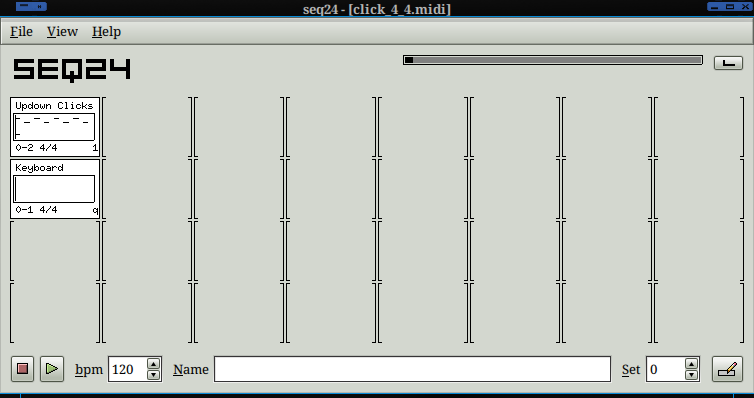
\includegraphics[scale=0.75]{seq24-first-screen.png}
   \caption{Seq24 Main Screen}
   \label{fig:seq24_main_screen}
\end{figure}

%  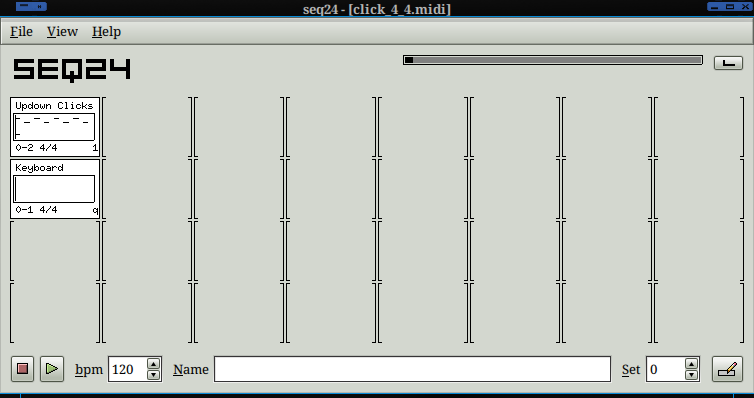
\includegraphics[scale=1.0]{seq24-first-screen.jpg}
%  That figure a bit out-of-date (it does not show the new "Part of"
%  feature), so we've replaced it with a new screen capture.
   
   Then the \textsl{Seq24} main window appears, as shown in
   \figureref{fig:seq24_main_screen}.

   The program is basically a loop playing machine with a 
   simple interface.  Before we describe this interface, it is useful to
   present some concepts.

% Important Concepts

%-------------------------------------------------------------------------------
% seq24_concepts
%-------------------------------------------------------------------------------
%
% \file        seq24_concepts.tex
% \library     Documents
% \author      Chris Ahlstrom
% \date        2015-07-19
% \update      2015-08-30
% \version     $Revision$
% \license     $XPC_GPL_LICENSE$
%
%     Provides the concepts.
%
%-------------------------------------------------------------------------------

\section{Concepts}
\label{sec:concepts}

   This section presents some useful concepts and definitions of terms as
   they are used in \textsl{Seq24}.

\subsection{Concepts / Terms}
\label{subsec:concepts_terms}

   This section doesn't provide comprehensive coverage of terms.  It
   covers mainly terms that puzzled the author at first or that are
   necessary to understand the \textsl{Seq24} program.

\subsubsection{Concepts / Terms / armed}
\label{subsubsec:concepts_terms_armed}

   \index{armed}
   An armed sequence is a sequence that will be heard.
   "Armed" is the opposite of "muted".
   Performing an \textsl{arm} operation in \textsl{Seq24} means clicking on
   an "unarmed" sequence in the patterns panel (the main window of
   \textsl{Seq24}).  An unarmed sequence will not be heard, and it
   has a white background.  When the sequence is \textsl{armed},
   it will be heard, and it has a black background.

   A sequence can be armed or unarmed in three ways:

   \begin{itemize}
      \item Clicking on the sequence/pattern box.
      \item Pressing the hot-key for that sequence/pattern box.
      \item Opening up the Song Editor and starting playback; the
            sequences arm/unarm depending on the layout of the
            sequences in the piano roll of the Song Editor.
   \end{itemize}

\subsubsection{Concepts / Terms / buss (bus)}
\label{subsubsec:concepts_terms_buss}

   \index{bus}
   \index{buss}
   A \textsl{buss} (also spelled "bus" these days) is an entity onto which
   MIDI events can be placed, in order to be heard or to affect the
   playback.

\subsubsection{Concepts / Terms / group}
\label{subsubsec:concepts_terms_group}

   \index{group}
   A \textsl{group} in \textsl{Seq24} is one of up to 32 previously-defined
   mute/unmute patterns in the active screen set.
   A group is a set of patterns that can toggle their playing state
   together.  Every group contains all 32 sequences in the active screen
   set.  This concept is similar to mute/unmute groups in hardware
   sequencers.

\subsubsection{Concepts / Terms / loop}
\label{subsubsec:concepts_terms_loop}

   \index{loop}
   \textsl{Loop}
   is a synonym for \textsl{pattern} or \textsl{sequence}, when used
   in existing \textsl{Seq24} documentation.
   Each loop is represented by a box in the Patterns window.

\subsubsection{Concepts / Terms / measures ruler}
\label{subsubsec:concepts_terms_measures_ruler}

   \index{measures ruler}
   The \textsl{measures ruler} is the bar at the top of the Song Editor
   arrangement window that shows the numbering of the measures in the song.
   Left and right markers can be dropped on this ruler to set durations to
   be played, looped, expanded, or collapsed.

   Note:
   \index{bar indicator}
   The original \textsl{Seq24} documentation calls this item the
   \textsl{bar indicator}.

\subsubsection{Concepts / Terms / MIDI clock}
\label{subsubsec:concepts_terms_midi_clock}

   \textsl{MIDI clock} is
   \index{midi clock}
   a MIDI timing reference signal used to synchronize pieces of equipment
   together. MIDI clock runs at a rate of 24 ppqn (pulses per quarter note).
   This means that the actual speed of the MIDI clock varies with the tempo
   of the clock generator (as contrasted with time code, which runs at a
   constant rate).

\subsubsection{Concepts / Terms / pattern}
\label{subsubsec:concepts_terms_pattern}

   A \textsl{Seq24} \textsl{pattern}
   \index{pattern}
   (also called a "sequence" or "loop")
   is a short unit of melody or rhythm in \textsl{Seq24},
   extending for a small number of measures (in most cases).
   Each pattern is represented by a box in the Patterns window.

   Each pattern is editable on its own.  All patterns can be layed out in
   a particular arrangement to generate a more complex song.

   \textsl{pattern} is a synonym for \textsl{loop} or \textsl{sequence}.
   It is our preferred term.

\subsubsection{Concepts / Terms / performance}
\label{subsubsec:concepts_terms_performance}

   In the jargon of \textsl{Seq24}, a
   \index{performance}
   \textsl{performance} is an organized collection of patterns.
   This collection of patterns is created using the Song Editor.

\subsubsection{Concepts / Terms / queue mode}
\label{subsubsec:concepts_terms_queue_mode}

   TODO:  \index{todo!queue definition}
   We need to figure out what "queue" refers to in the documentation, what
   do the "temporary queue" and "permanent queue" are, and what the "keep
   queue" functionality is used for.

\subsubsection{Concepts / Terms / screen set}
\label{subsubsec:concepts_terms_screen_set}

   The \textsl{screen set}
   \index{screen set}
   is a set of patterns that fit within the 8x4 grid of loops/pattern in the
   Patterns panel.
   \textsl{Seq24} supports multiple screens sets, and a name can be given to
   each for clarity.

\subsubsection{Concepts / Terms / sequence}
\label{subsubsec:concepts_terms_sequence}

   \index{sequence}
   \textsl{Sequence} seems to be
   another synonym for \textsl{pattern}, used in some of the \textsl{Seq24}
   documentation.  \textsl{Loop} is another synonym.
   Each sequence is represented by a box in the Patterns window.

\subsubsection{Concepts / Terms / snapshot}
\label{subsubsec:concepts_terms_snapshot}

   \index{snapshot}
   A \textsl{Seq24} \textsl{snapshot} is simply a briefly preserved state.
   One can press a snapshot key, change the state of the patterns for live
   playback, and then release the snapshot key to revert to the state when
   it was first pressed.  (Might call it a "revert" key, instead.)

\subsubsection{Concepts / Terms / song}
\label{subsubsec:concepts_terms_song}

   \index{song}
   A \textsl{song} is a collection of patterns in a specific layout, as
   assembled via the Song Editor window.

%-------------------------------------------------------------------------------
% vim: ts=3 sw=3 et ft=tex
%-------------------------------------------------------------------------------


% Menu

%-------------------------------------------------------------------------------
% seq24_menu
%-------------------------------------------------------------------------------
%
% \file        seq24_menu.tex
% \library     Documents
% \author      Chris Ahlstrom
% \date        2015-07-19
% \update      2015-07-20
% \version     $Revision$
% \license     $XPC_GPL_LICENSE$
%
%     Provides the Menu section of seq24-user-manual.tex.
%
%-------------------------------------------------------------------------------

\section{Menu}
\label{sec:seq24_menu}

   The \textsl{Seq24} menu, as seen at the top of
   \figureref{fig:seq24_main_screen},
   is fairly simple, but it is important to understand the
   structure of the menu entries.

\subsection{Menu / File}
\label{subsec:seq24_menu_file}

   The \textbf{File} menu is used to save and load standard 
   MIDI files.  It should be able to handle any 
   Format 1 standard files that any other sequencer 
   is capable of exporting.  

   The \textsl{Seq24}
   menu entry contains the sub-items shown in
   \figureref{fig:seq24_menu_file_items}.
   The next few sub-sections discuss the sub-items in the 
   \textsl{File} sub-menu.

\begin{figure}[H]
   \centering 
   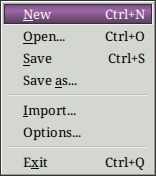
\includegraphics[scale=1.0]{menu/menu_file.png}
   \caption{Seq24 File Menu Items}
   \label{fig:seq24_menu_file_items}
\end{figure}

   \begin{enumber}
      \item \textbf{New}
      \item \textbf{Open...}
      \item \textbf{Save}
      \item \textbf{Save As...}
      \item \textbf{Import...}
      \item \textbf{Options...}
      \item \textbf{Exit}
   \end{enumber}

\subsection{Menu / File / New}
\label{subsec:menu_file_new}

   The \textbf{New} menu entry clears out any current song and patterns,
   along one to create news ones from scratch.

\subsubsection{Menu / File / Open}
\label{subsubsec:seq24_menu_file_open}

   The \textbf{Open} menu entry opens a song that had been saved previously.
   It opens up a standard GTK+ file dialog.

\begin{figure}[H]
   \centering 
   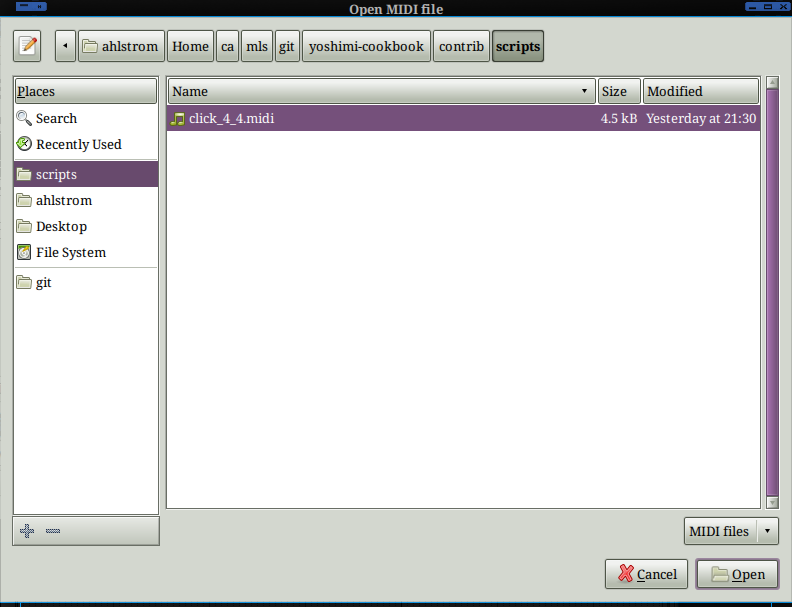
\includegraphics[scale=0.50]{menu/menu_file_open.png}
   \caption{File Open}
   \label{fig:seq24_menu_file_open}
\end{figure}

\subsubsection{Menu / File / Save (As)}
\label{subsubsec:menu_file_open_save_as}

   The \textbf{Save As} menu entry saves a song under a different name.
   It opens up a standard GTK+ file dialog.

\begin{figure}[H]
   \centering 
   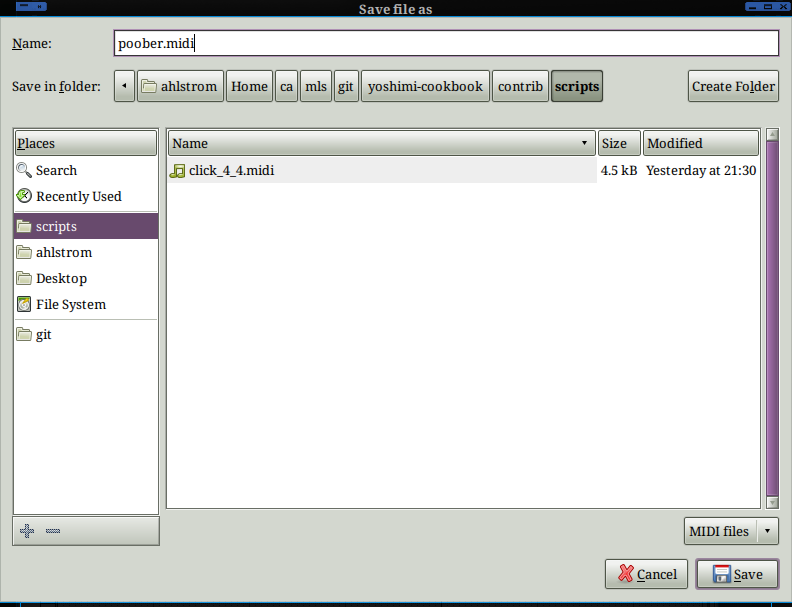
\includegraphics[scale=0.50]{menu/menu_file_save_as.png}
   \caption{File Save As}
   \label{fig:seq24_menu_file_save_as}
\end{figure}

   The \textbf{Save} menu entry saves the song under its current name.
   If there is no current name, then
   it opens up a standard GTK+ file dialog.

\subsubsection{Menu / File / Import}
\label{subsubsec:seq24_menu_file_import}

   The \textbf{Import} menu entry allows one to import a MIDI file
   into a pattern.

\begin{figure}[H]
   \centering 
   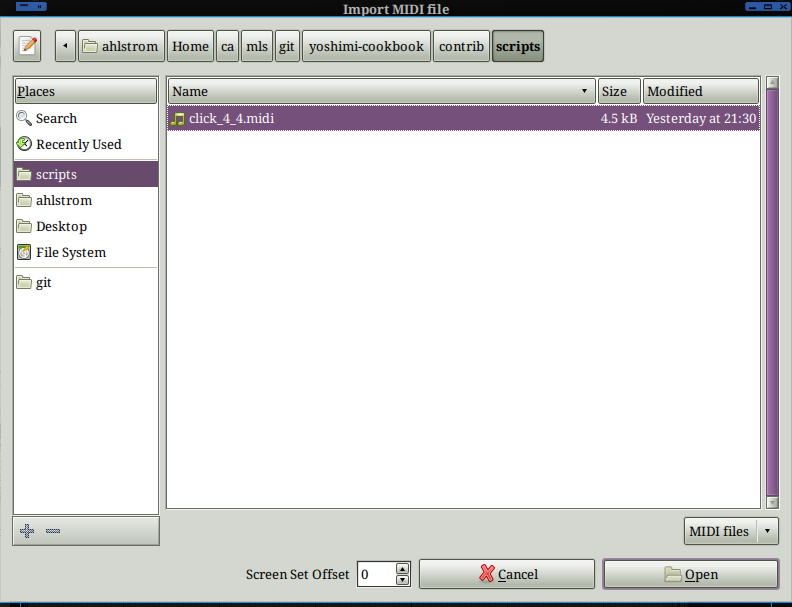
\includegraphics[scale=0.75]{menu/menu_file_import.png}
   \caption{File Import}
   \label{fig:seq24_menu_file_import}
\end{figure}

   When imported, each track, whether a music track or an information track,
   is entered into its own loop/pattern box.  The import operation can
   handle reasonably complex files, as shown in the following diagram, which
   shows an import of the \texttt{contrib/b4uacuse.mid} file, which contains
   a transcription of an Eric Clapton tune that we'd made over 20 
   years ago and had uploaded to the \textsl{GEnie} network service.

\begin{figure}[H]
   \centering 
   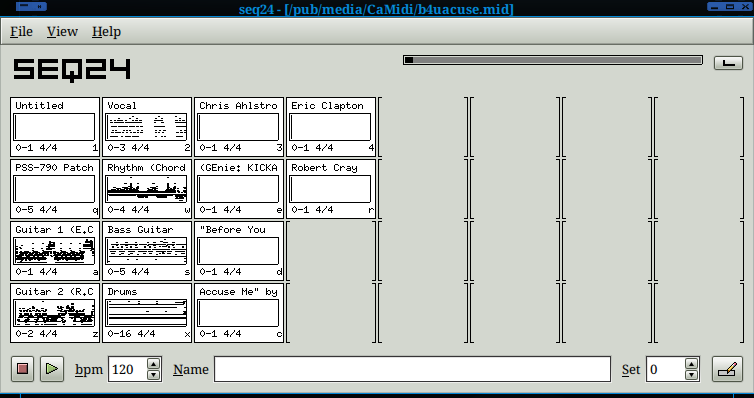
\includegraphics[scale=0.50]{menu/imported_midi_song.png}
   \caption{File Import}
   \label{fig:seq24_imported_midi_song}
\end{figure}

   Unfortunately, this song was created before the days of General MIDI.
   It is scored for the Yamaha PSS-790 consumer-level synthesizer.
   One can use our MIDI-conversion project (see reference \cite{midicvt}) 
   to convert it to General MIDI format, including General MIDI drums.

\subsubsection{Menu / File / Options}
\label{subsubsec:seq24_menu_file_options}

   This menu provides a number of settings in one tabbed dialog, shown in
   the figure below.
   This window allows us to select which sequence gets the MIDI
   clock, and which incoming MIDI events control the sequencer.

\paragraph{Menu / File / Options / MIDI Clock}
\label{paragraph:seq24_menu_file_options_midi_clock}

   Provides a way to send the MIDI clock to one or more of the
   \textsl{Seq24} output busses.
   It is used to configure to what busses the MIDI clock gets dumped.

\begin{figure}[H]
   \centering 
   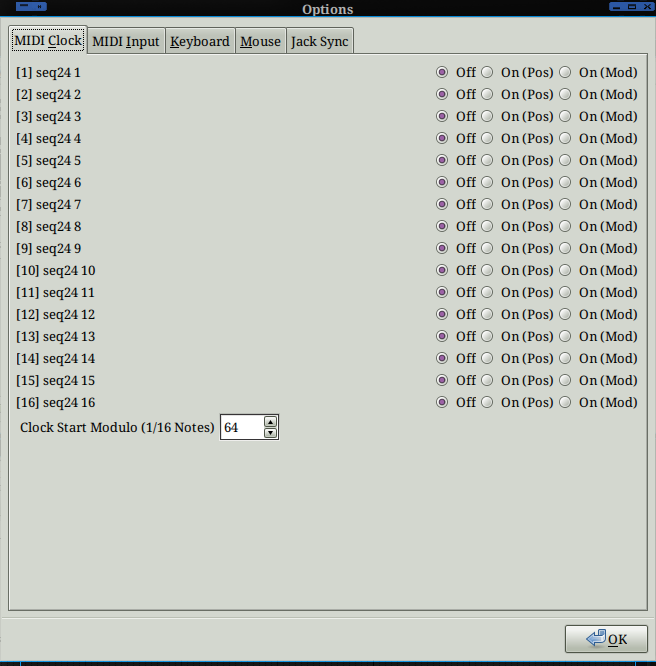
\includegraphics[scale=0.75]{menu/menu_file_options_midi_clock.png}
   \caption{File Options MIDI Clock}
   \label{fig:seq24_menu_file_options_midi_clock}
\end{figure}

   The following elements are present in this dialog:

   \begin{enumber}
      \item \textbf{Buss Name}
      \item \textbf{Off}
      \item \textbf{On (Pos)}
      \item \textbf{On (Mod)}
      \item \textbf{Clock Start Modulo}
   \end{enumber}

   \setcounter{ItemCounter}{0}      % Reset the ItemCounter for this list.

   \itempar{Buss Name}{midi clock!buss name}
   These labels indicate the output busses of \textsl{Seq24}.
   They range from \textbf{[1] seq24 1}
   to \textbf{[16] seq24 16}.

   \itempar{Off}{midi clock!off}
   This setting disables the MIDI clock for the given output buss.

   \itempar{On (Pos)}{midi clock!on (pos)}
   The MIDI clock will be sent to this buss.
   MIDI Song Position and MIDI Continue will be sent if playback is starting
   at greater than tick 0 in Song mode.  Otherwise, MIDI Start will be sent.

   \itempar{On (Mod)}{midi clock!on (mod)}
   The MIDI clock will be sent to this buss.
   MIDI Start will be sent and clocking will begin
   once the Song Position has reached the start modulo of the specified size
   (see the next item's description).
   This setting is used for gear that does not respond to Song Position.

   \itempar{Clock Start Modulo}{midi clock!clock start modulo}
   Clock Start Modulo (1/16 Notes).
   This value starts at 1 and ranges on upward to 16384.
   It  defaults to 64.
   It is used by the \textbf{On (Mod)} setting discussed above.

\paragraph{Menu / File / Options / MIDI Input}
\label{paragraph:seq24_menu_file_options_midi_input}

   The only item in this tab is the single MIDI input buss provided
   by \textsl{Seq24}:  \textbf{[0] seq24 0}.

\begin{figure}[H]
   \centering 
   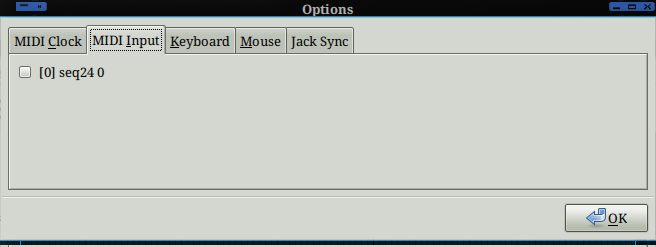
\includegraphics[scale=0.75]{menu/menu_file_options_midi_input_condensed.png}
   \caption{File Options MIDI Input (Condensed View)}
   \label{fig:seq24_menu_file_options_midi_input}
\end{figure}

   This item, if checked allows \textbf{Seq24} to be used to record MIDI
   information from another source, or pass it through to the output busses
   that are configured to allow pass-through.

\paragraph{Menu / File / Options / Keyboard }
\label{paragraph:seq24_menu_file_options_keyboard}

   \textsl{Seq24}, as befits a professional product, allows extensive use of
   keyboard shortcuts to make operations go faster than when using a mouse.

\begin{figure}[H]
   \centering 
   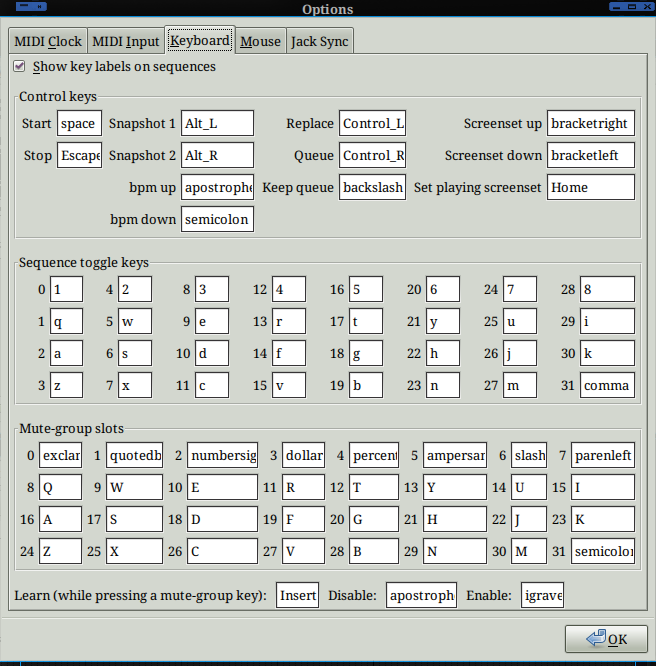
\includegraphics[scale=0.75]{menu/menu_file_options_keyboard.png}
   \caption{File Options Keyboard}
   \label{fig:seq24_menu_file_options_keyboard}
\end{figure}

   We won't attempt to cover every user-interface item in this dialog, just
   the categories.

   \begin{enumber}
      \item \textbf{Show key labels on sequences}
      \item \textbf{Control keys}
      \item \textbf{Sequence toggle keys}
      \item \textbf{Mute-group slots}
      \item \textbf{Learn}
      \item \textbf{Disable}
      \item \textbf{Enable}
   \end{enumber}

   \setcounter{ItemCounter}{0}      % Reset the ItemCounter for this list.

   \itempar{Show key labels on sequence}{keyboard!show labels}
   This item, if enabled, shows the key labels in the lower-right corner of
   each loop/pattern in the Patterns window.

   \itempar{Control keys}{keyboard!control keys}
   This block of fields provides shortcut keys for many operations of
   \textsl{Seq24}.

   \begin{enumber}
      \item \textbf{Start}.
         Key: \index{keys!space} \textbf{space}.
      \item \textbf{Stop}.
         Key: \index{keys!esc} \textbf{Escape}.
      \item \textbf{Snapshot 1}.
         Key: \index{keys!alt-L} \textbf{Alt\_L}.
      \item \textbf{Snapshot 2}.
         Key: \index{keys!alt-R} \textbf{Alt\_R}.
      \item \textbf{bpm up}.
         Key: \index{keys!apostrophe} \textbf{apostrophe}.
      \item \textbf{bpm down}.
         Key: \index{keys!;} \textbf{semicolon}.
      \item \textbf{Replace}.
         Key: \index{keys!ctrl-L} \textbf{Control\_L}.
      \item \textbf{Queue}.
         Key: \index{keys!ctrl-R} \textbf{Control\_R}.
      \item \textbf{Keep queue}.
         Key: \index{keys!backslash} \textbf{backslash}.
      \item \textbf{Screenset down}.
         Key: \index{keys![} \textbf{bracketleft}.
      \item \textbf{Screenset up}.
         Key: \index{keys!]} \textbf{bracketright}.
      \item \textbf{Set playing screenset}.
         Key: \index{keys!home} \textbf{Home}.
   \end{enumber}

   Note that some of the keys have positional mnemonic value.  For example,
   for BPM control, the semicolon is at the left (down), and the apostrophe
   is at the right (up).

   TODO: One thing we need to figure out is just what this "snapshot"
   feature provides.  Another thing is the "queue" and "keep queue"
   features.

   \itempar{Sequence toggle keys}{keyboard!sequence toggle keys}
   Each of these keys toggles the playing/muting of one of the 32
   loop/pattern boxes.  These keys are layed out logically on the keyboard,
   and can also be shown in each loop/pattern box.  No need to list them all
   here!

   \itempar{Mute-group slots}{keyboard!mute-group slots}
   Each of these keys operates on the mute-grouping of one of the 32
   loop/pattern boxes.  These keys are layed out logically on the keyboard,
   and can also be shown in each loop/pattern box.  No need to list them all
   here!

   TODO: One thing we need to discover is just what this mute-grouping
   means.

   \itempar{Learn}{keyboard!learn}
   Learn (while pressing a mute-group key).
   This items sets the key used to initiate a learn mode.
   It is the \textbf{Insert} key by default.

   \itempar{Disable}{keyboard!disable}
   TODO: What gets disabled?
   It is the \textbf{apostrophe} key by default.

   \itempar{Enable}{keyboard!enable}
   TODO: What gets enabled?
   It is the \textbf{igrave} (back-tick) key by default.

   There is much to learn about this learn/enable/disable triad!

\paragraph{Menu / File / Options / Mouse }
\label{paragraph:seq24_menu_file_options_mouse}

   This item selects the mouse-interaction method.

\begin{figure}[H]
   \centering 
   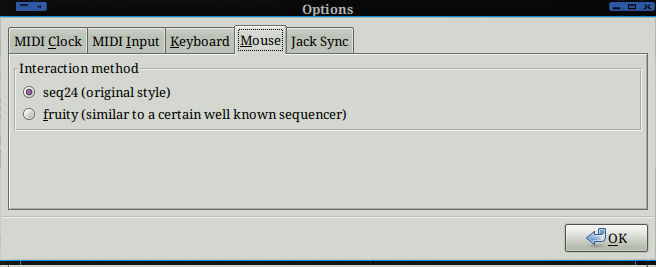
\includegraphics[scale=0.75]{menu/menu_file_options_mouse_condensed.png}
   \caption{File Options Mouse (Condensed View)}
   \label{fig:seq24_menu_file_options_mouse}
\end{figure}

   The default method is \textbf{seq24 (original style)}.
   The alternate method is \textbf{fruity (similar to a certain well known
   sequencer)}.

   The alternate method is presumably that of the \textsl{Fruity Loops}
   (now \textsl{FL Studio}) sequencer.
   
   TODO: But we currently have no idea what that means.

\paragraph{Menu / File / Options / Jack Sync }
\label{paragraph:seq24_menu_file_options_jack_sync}

   This tab sets up options for JACK synchronization.

\begin{figure}[H]
   \centering 
   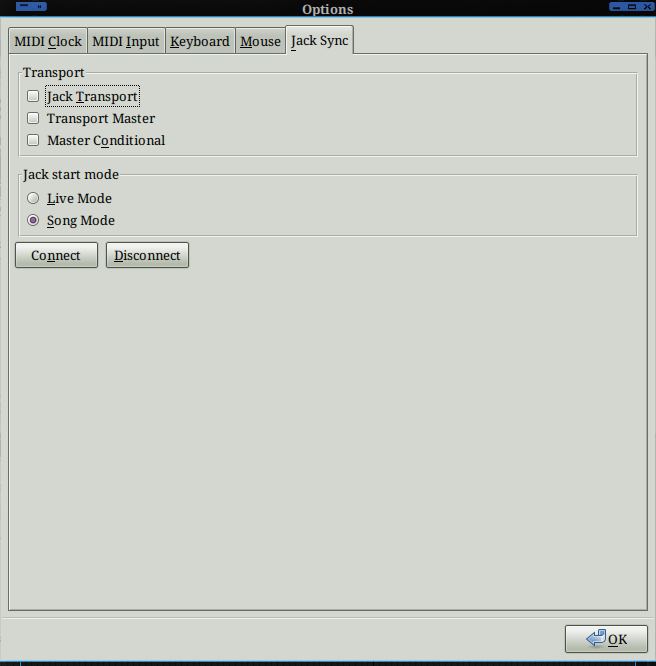
\includegraphics[scale=0.75]{menu/menu_file_options_jack_sync.png}
   \caption{File Options Jack Sync}
   \label{fig:seq24_menu_file_options_jack_sync}
\end{figure}

   \begin{enumber}
      \item \textbf{Transport}
      \item \textbf{Jack start mode}
      \item \textbf{Connect}
      \item \textbf{Disconnect}
   \end{enumber}

   \setcounter{ItemCounter}{0}      % Reset the ItemCounter for this list.

   \itempar{Transport}{jack sync!transport}
   This items collects the following settings:

   \begin{itemize}
      \item \textbf{Jack Transport}.
         \index{JACK!transport}
         Enables synchronization with JACK Transport.
      \item \textbf{Transport Master}.
         \index{JACK!transport master}
         \textsl{Seq24} will attempt to serve as the JACK Master.
      \item \textbf{Master Conditional}.
         \index{JACK!master conditional}
         \textsl{Seq24} will fail to serve as the JACK Master if there is
         already a Master set.
   \end{itemize}

   \itempar{Transport}{jack sync!transport}
   This items collects the following settings:

   \begin{itemize}
      \item \textbf{Live Mode}.
         \index{JACK!live mode}
         Playback will be in live mode.  Use this option to allow muting and
         unmuting of loops.
      \item \textbf{Song Mode}.
         \index{JACK!song mode}
         Playback will use only the Song Editor's data.
   \end{itemize}

   \itempar{Connect}{jack sync!connect}
   Connect to JACK Sync.

   \itempar{Disconnect}{jack sync!disconnect}
   Disconnect from JACK Sync.

\subsection{Menu / View}
\label{subsec:seq24_menu_view}

   This menu item has only one entry, \textbf{Song Editor}, 
   which is already covered by a button at the bottom of the Patterns
   window.  Selecting this item bring up the Song Editor window.

\subsection{Menu / Help About...}
\label{subsec:seq24_menu_about}

   This menu entry shows the "About" dialog.

\begin{figure}[H]
   \centering 
   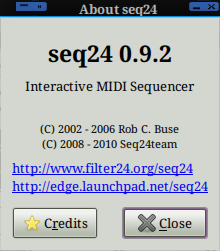
\includegraphics[scale=0.75]{menu/menu_help_about.png}
   \caption{Help About}
   \label{fig:seq24_menu_help_about}
\end{figure}

   That dialog provides access to the credits for the program, including the
   authors and the project documentor.

\begin{figure}[H]
   \centering 
   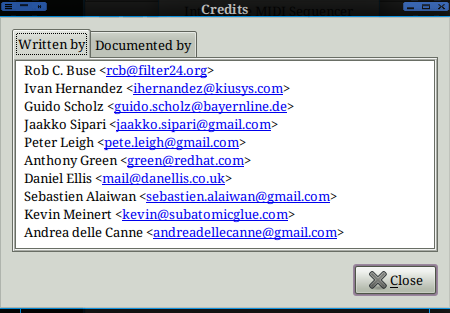
\includegraphics[scale=0.75]{menu/menu_help_credits.png}
   \caption{Help Credits}
   \label{fig:seq24_menu_help_credits}
\end{figure}

   Shows who has worked on the program, with the original author at the top
   of the list.

\begin{figure}[H]
   \centering 
   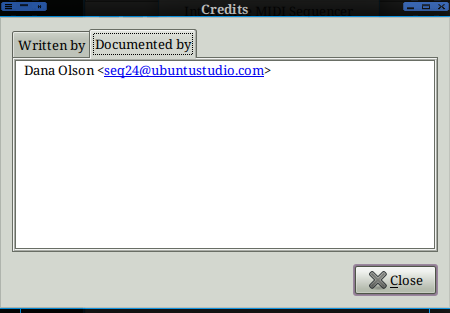
\includegraphics[scale=0.75]{menu/menu_help_doc.png}
   \caption{Help Documentation}
   \label{fig:seq24_menu_help_doc}
\end{figure}

   Shows who has documented this project.  Say, maybe "we" can get "our"
   name their someday!  :-)


%-------------------------------------------------------------------------------
% vim: ts=3 sw=3 et ft=tex
%-------------------------------------------------------------------------------


% Patterns Panel

%-------------------------------------------------------------------------------
% seq24_patterns_panel
%-------------------------------------------------------------------------------
%
% \file        seq24_patterns_panel.tex
% \library     Documents
% \author      Chris Ahlstrom
% \date        2015-07-19
% \update      2015-08-30
% \version     $Revision$
% \license     $XPC_GPL_LICENSE$
%
%     Provides the concepts.
%
%-------------------------------------------------------------------------------

\section{Patterns Panel}
\label{sec:seq24_patterns_panel}

   \textsl{Seq24} works with the idea of patterns (loops) that are repeated
   all along a song.  One composes and edits small patterns, and combines
   them to create a full song.  This is a powerful way to work, and makes
   one productive within an hour.

   The \textsl{Seq24 Patterns Panel} is the main window of \textsl{Seq24}.
   See \figureref{fig:seq24_main_screen}.
   It is also called the "main window" or the "patterns window".
   It is here one manages a set of patterns
   (see \sectionref{subsubsec:concepts_terms_screen_set}),
   manages the configuration, and opens the pattern or song editors.

   For exposition, we break it into a top panel, a pattern panel, and a
   bottom panel.  Note that the \textsl{Seq24} main menu is discussed in
   \sectionref{sec:seq24_menu}.

\subsection{Patterns / Top Panel}
\label{subsec:seq24_patterns_panel_top}

   The top panel of the Pattern window is simple, consisting of the name of
   the program and a couple of controls.

\begin{figure}[H]
   \centering 
   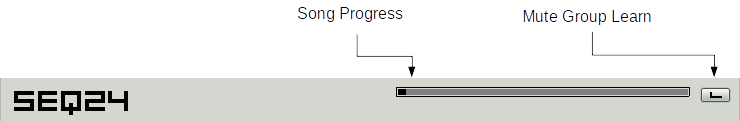
\includegraphics[scale=0.75]{pattern-window-top-panel-items.png}
   \caption{Patterns Panel, Top Panel Items}
   \label{fig:pattern_window_top_panel_items}
\end{figure}

   \begin{enumber}
      \item \textbf{Song Progress}
      \item \textbf{Mute Group Learn}
   \end{enumber}

   \setcounter{ItemCounter}{0}      % Reset the ItemCounter for this list.

   \itempar{Song Progress}{pattern!progress}
   \index{song!progress}
   \index{song!"main time"}
   The \textbf{Song Progress} bar is also known as the "main time" bar.
   This bar shows a number of small black cursors ("pills") that show the
   progress of the song through the various patterns.  For short patterns,
   the progress is fast.  For patterns that last longer, the progress is
   slow.  This field shows that something is going on.  It can also indicate
   the relative lengths of the various patterns.
 
   Note that the individual pattern boxes in the main panel have their own
   moving progress cursor, a tall thin line in each box.  Unfortunately,
   this bar moves along even in patterns that have no events, only meta
   items such as the track name.

   \itempar{Mute Group Learn}{pattern!mute group learn}
   \index{"L" button}
   This button is also known as the "L" button.
   Click this button, and then press a mute-group key
   to store the mute-state of the patterns in that key.

   See the \textbf{File / Options / Keyboard} menu entry to bring up the
   dialog showing the available mute-group keys and the corresponding
   hot-key for the "L" button.

   \index{group!toggle}
	One can toggle the playing status of up to 32 previously
	defined mute/unmute patterns (groups) in the active screen
	set, similar to hardware sequencers.
	This toggling is done either by one of the \textsl{group toggle} keys
	or by a MIDI controller, both assigned in the
   \texttt{~/.seq24rc} file.
	A mute/unmute pattern (group) is stored by holding a
   \index{group!learn}
   \textsl{group learn} key (\texttt{Insert} by default) while pressing the
   corresponding \textsl{group toggle} key.
	There are also keys assigned to turn on/off the group
	functionality.

\subsection{Patterns / Main Panel}
\label{subsec:seq24_patterns_panel_main}

   The main panel of the Patterns window provides a grid of empty boxes,
   each box delimited by brace-like lines at left and right.
   Each filled box represents a loop or pattern.
   One sees only 32 loops at a time in the main panel (but more 32
   loops can be supported by \textsl{Seq24}.
   \index{screen set}
   This group of 32 loops is called a "screen set", as discussed in
   \sectionref{subsubsec:concepts_terms_screen_set}.
   One can switch between sets
   by using the
   \index{keys![}
   \texttt{[} and
   \index{keys!]}
   \texttt{]} keys on the keyboard, or by using
   the spin-widget-driven, labelled \textbf{Set} interface item.
   There are a total of 32 sets, for a total of
   1024 loops/patterns. 

\begin{figure}[H]
   \centering 
   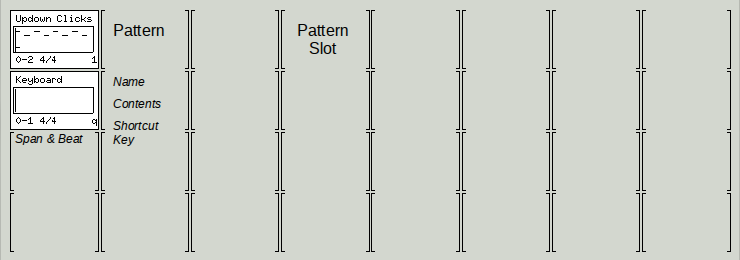
\includegraphics[scale=0.75]{pattern-window-main-panel-items.png}
   \caption{Patterns Panel, Main Panel Items}
   \label{fig:pattern_window_main_panel_items}
\end{figure}

   \begin{enumber}
      \item \textbf{Pattern Slot}
      \item \textbf{Pattern}
   \end{enumber}

\subsubsection{Pattern Slot}
\label{subsubsec:seq24_patterns_pattern_slot}

   \index{pattern!slot}
   An empty box is a slot for a pattern.
   \index{pattern!right click}
   By right-clicking on an empty box one brings up a menu to create
   a new loop, as well as some other operations:

\begin{figure}[H]
   \centering 
   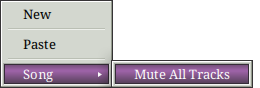
\includegraphics[scale=0.75]{pattern/pattern-empty-right-click-menu.png}
   \caption{Empty Pattern, Right-Click Menu}
   \label{fig:pattern_window_empty_right_click}
\end{figure}

   \begin{enumber}
      \item \textbf{New}
      \item \textbf{Paste}
      \item \textbf{Song / Mute All Tracks}
   \end{enumber}

   \setcounter{ItemCounter}{0}      % Reset the ItemCounter for this list.

   \itempar{New}{pattern!new}
   Creates a new loop or pattern.
   Clicking this menu entry fills in the empty box with an untitled
   pattern, and brings up the Pattern Editor
   so that one can fill in the new pattern.

   \itempar{Paste}{pattern!paste}
   Pastes a loop or pattern that was previously copied.

   \itempar{Song / Mute All Tracks}{pattern!mute all}
   This item is the one item in the \textbf{Song} context menu;
   it mutes all tracks (or loops/patterns).  (We are not clear
   on exactly what it does.  There is no change in visible
   status of any of the patterns in the patterns-panel.)

\subsubsection{Pattern}
\label{subsubsec:seq24_patterns_pattern_filled}

   A filled pattern slot is referred to informally as a pattern.
   A pattern is shown in the Pattern windows as a filled box with the
   following items of information in it:

   \begin{itemize}
      \item \textbf{Name}.
         \index{pattern!name}
         This line contains the name or title of the pattern, to help
         reference it when juggling a number of patters.
      \item \textbf{Contents}.
         \index{pattern!contents}
         The contents of the pattern provide a fairly detailed and
         distinguishable representation of the notes or events in the
         pattern.  Also, when the song is playing, a vertical bar cursor
         tracks the position of the playback of the pattern or loop; it
         returns to the beginning of the box every time that pattern starts
         over again.
         \textbf{Bug:}
         \index{bugs!empty pattern scrolls}
         However, an imported empty pattern will still (needlessly) scroll;
         perhaps such patterns can be marked as inactive.
      \item \textbf{Bus-Channel}.
         \index{pattern!bus-channel}
         This pair of numbers shows the the MIDI buss number, a dash, and
         the MIDI channel number.
         For example, "0-2" means MIDI buss 0, channel 2.
      \item \textbf{Beat}.
         \index{pattern!beat}
         This pair of numbers is the standard time-signature of the pattern,
         such as "4/4" or "3/4".  The first number is the beats-per-measure,
         and the second is the size of the beat, here, a quarter note.
      \item \textbf{Shortcut Key}.
         If the display of shortcut keys is enabled (see
         \sectionref{paragraph:seq24_menu_file_options_keyboard}),
         then the key noted in the lower-right corner of the pattern can be
         pressed to toggle the mute/unmute status of that pattern.
         This action is an alternative to left-clicking on the pattern.
      \item \textbf{Progress Cursor}.
         At the left of each box is a vertical line, waiting for playback to
         start so that it can move through the pattern, again and again.
   \end{itemize}

   \index{pattern!left click}
   Left-clicking on an filled pattern box will toggle the status of the
   pattern between muted (white background) and unmuted (black background).
   If the song is playing via the main window, toggling this status makes
   the pattern stop playing or start playing.  Note that the armed status
   can also be toggled using hot-keys.

   Also note that the pattern boxes will toggle between the muted/unmuted
   states as the music plays, and the pattern is active or inactive at the
   point of playback, if the Song Editor is the active window and was used
   to start the playback.

   \index{pattern!right click}
   By right-clicking on an already-filled box, one brings up a menu
   to allow one to edit a existing one, or perform a few other actions
   specified in the context menu.  Here is that menu:

\begin{figure}[H]
   \centering 
   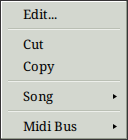
\includegraphics[scale=0.75]{pattern/pattern-right-click-menu.png}
   \caption{Existing Pattern, Right-Click Menu}
   \label{fig:pattern_window_right_click}
\end{figure}

   Here one can choose to edit the pattern, cut and copy the pattern,
   set the MIDI bus/channel, and more.
   One can also clear all performance data for the pattern.
   
   \begin{enumber}
      \item \textbf{Edit...}
      \item \textbf{Cut}
      \item \textbf{Copy}
      \item \textbf{Song/}
      \item \textbf{Midi Bus/}
   \end{enumber}

   \setcounter{ItemCounter}{0}      % Reset the ItemCounter for this list.

   \itempar{Edit}{pattern!edit}
   Edits an existing loop or pattern.
   Clicking this menu entry brings up the Pattern Editor
   so that one can modify the existing pattern.
   See \figureref{fig:pattern_edit_window}.

   \itempar{Cut}{pattern!cut}
   Deletes and copies an existing loop or pattern.

   \textbf{Bug:}
   \index{bugs!pattern cut doesn't work}
   This operation seems to have no effect.  The loop or pattern remains in
   place.

   \itempar{Copy}{pattern!copy}
   Copies an existing loop or pattern.
   The pattern can then be pasted elsewhere in the Patterns panel.
   See \sectionref{subsubsec:seq24_patterns_pattern_slot}.

   \itempar{Song}{pattern!song}
   Clicking this menu entry brings up a small popup menu:

\begin{figure}[H]
   \centering 
   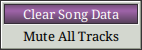
\includegraphics[scale=0.75]{pattern/pattern-menu-song.png}
   \caption{Existing Pattern, Right-Click Menu, Song}
   \label{fig:pattern_window_right_click_song}
\end{figure}

   \begin{enumber}
      \item \textbf{Clear Song Data}
      \item \textbf{Mute All Tracks}
   \end{enumber}

   \setcounter{ItemCounter}{0}      % Reset the ItemCounter for this list.

   \itempar{Clear Song Data}{pattern!clear song data}
   Selecting this filled-box right-click menu item causes that box's
   loop/pattern to be removed from the song.  This means
   that it disappears from the Song Editor window, and so will not
   be played when the song plays.

   \itempar{Mute All Tracks}{pattern!mute all tracks}
   Selecting this filled-box right-click menu item causes...
   TODO.  \index{todo!how mute all tracks works}
   Cannot yet see that this does anything, NEEDS EXPERIMENTATION.

   \itempar{Midi Bus}{pattern!midi bus}
   Selecting this filled-box right-click menu item brings up a list
   of the 16 MIDI output busses that \textsl{Seq24} supports:

\begin{figure}[H]
   \centering 
   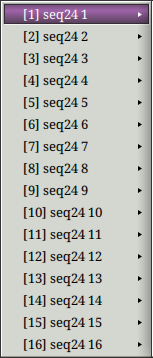
\includegraphics[scale=0.75]{pattern/pattern-menu-midi-bus.png}
   \caption{Existing Pattern, Right-Click Menu, MIDI Output Busses}
   \label{fig:pattern_window_right_click_midi_bus}
\end{figure}

   For each of these buss items, another pop-up menu allows one
   to specify the MIDI output port for that buss:

\begin{figure}[H]
   \centering 
   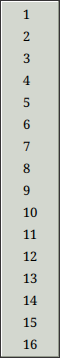
\includegraphics[scale=0.75]{pattern/pattern-menu-midi-bus-numbers.png}
   \caption{Existing Pattern, Right-Click Menu, MIDI Bus Ports}
   \label{fig:pattern_window_right_click_midi_bus_numbers}
\end{figure}

\subsubsection{Pattern Keys and Click}
\label{subsubsec:seq24_patterns_pattern_keys_and_clicks}

   This section recapitulates all the clicks and keys that perform actions
   in the Pattern windows.  Some additional clicks and keys are noted here
   as well.

\paragraph{Pattern Keys}
\label{paragraph:seq24_patterns_pattern_keys}

   Each pattern in the patterns panel can have a hot-key associated with it.
   \index{keys!hot-keys}

   \index{keys!pattern toggles}
   For each pattern, hitting its assigned keyboard key will
   also toggle its status between muted/unmuted (armed/unarmed).
   Below is the default grid that is
   mapped to the loops/patterns on the screen set.
   This grid can be changed in the Keyboard options tab, and is
   saved in the \textsl{keyboard-control} section of the
   \texttt{~/.seq24rc} file.

   \begin{verbatim}
     [ 1   ][ 2   ][ 3   ][ 4   ][ 5   ][ 6   ][ 7   ][ 8   ]
     [ q   ][ w   ][ e   ][ r   ][ t   ][ y   ][ u   ][ i   ]
     [ a   ][ s   ][ d   ][ f   ][ g   ][ h   ][ j   ][ k   ]
     [ z   ][ x   ][ c   ][ v   ][ b   ][ n   ][ m   ][ ,   ]
   \end{verbatim}

   These characters are shown in the lower right corner of each
   pattern, as an aid to memory.

   These hot-keys can be modified

   \index{keys![}
   \index{keys!decrement set}
   The \texttt{[} and
   \index{keys!]}
   \index{keys!increment set}
   \texttt{]} keys on the keyboard
   switch between sets, either decrementing or incrementing the set number.

   The left and right Alt keys are, by default, set up in the
   \textbf{File / Options / Keyboard / Snapshot 1} and
   \textbf{Snapshot 2} fields to be used as "snapshot" keys.

   When one of these snapshot keys is pressed, the state of the patterns
   (which ones are armed versus unarmed) is instantly saved.  While the
   snapshot key is pressed, on can then change the state of the patterns to
   change how the song plays back.  When the snapshot key is released, the
   original saved state of the patterns is restored.

   \index{keys!alt}
   Holding \texttt{Alt} will save the state of playing patterns and restore
   them when \texttt{Alt} is lifted.

   The handling of \texttt{Alt} is generally taken over by the window
   manager, so there could be a need to change these items to some other
   keys.

%  \index{keys!left ctrl alt}
%  Holding \texttt{Left Ctrl} and \texttt{Alt} at the same time will enable
%  one to flip over to new patterns briefly and then flip right back upon
%  lifting \texttt{Alt}.  Not yet sure exactly what this means.

   \index{keys!right ctrl}
   \index{keys!queue}
   \index{queue!temporary}
	Holding \texttt{Right Ctrl} will queue a on/off toggle for a 
	sequence when the loop ends. This is the "queue" functionality.
   This means that the change in state of the pattern will not take hold
   immediately, but will kick in when the pattern restarts.

   This pending state is indicated by coloring the central box of the
   pattern grey, as shown in the following figure.

\begin{figure}[H]
   \centering 
   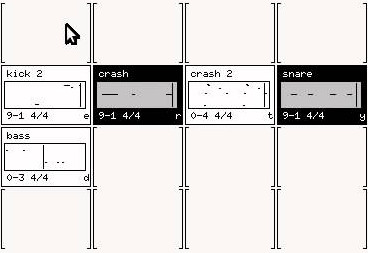
\includegraphics[scale=0.75]{pattern/seq24-queueing-coloration.jpg}
   \caption{Example of Pattern Coloration when Queued}
   \label{fig:seq24_queueing_coloration}
\end{figure}

   Queue also works for mute/unmute 
	patterns (groups); in this case every sequence will toggle 
	its status after its individual loop end. 

   Of course, the Ctrl key is used to manage the GUI (e.g. Ctrl-q will
   unceremoniously quit the application), so one will usually want to change
   this key to something else in the
   \textbf{File / Options / Keyboard / Queue} field.
   The Super key (i.e. the Mod4 or Windows key) is a good candidate to
   replace the right Ctrl key.

   Note that there is also a "Replace" key, which is the left Ctrl key by
   default.  We still need to document this functionality.
   \index{todo!replace key}.

   \index{keys!backslash}
   \index{keys!keep queue}
   \index{queue!permanent}
   \index{queue!keep queue}
	Pressing the "keep queue" key (by default, the backslash key)
   assigned in the \textsl{~/.seq24rc} file
	activates permanent queue mode until you use the temporary 
	queue function again pressing \texttt{Right Ctrl}. 

   This key can be changed in the
   \textbf{File / Options / Keyboard / Keep queue} field.

   There are more keys defined in the \textbf{Keyboard} dialog, and it is
   worth figuring out what they do, if not documented here.
   For a couple of short, but good, tutorials about using arming, queueing,
   and snapshots, see references \cite{wootangent1}
   and \cite{wootangent2}.

\paragraph{Pattern Clicks}
\label{paragraph:seq24_patterns_pattern_Clicks}

   \index{pattern!left click}
   \index{pattern!mute toggle}
   Left-clicking on a pattern-filled box will change its state
   \index{pattern!mute}
   \index{pattern!unmute}
   from muted (white background) to playing (black background) when
   the sequencer is running.

   \index{pattern!left ctrl left click}
   \index{keys!left ctrl}
   Holding down \texttt{Left Ctrl} while selecting a pattern
   with a left click will mute all other patterns and turn on the selected
   pattern.

   \index{pattern!left click-drag}
   By clicking and holding the left mouse button on a pattern,
   one can drag it to a new location on the grid.  The box
   will disappear while dragged, and reappear in the new location when
   dropped.  However, note that a pattern cannot be dragged if its
   Pattern Editor window is open.

   \index{pattern!right click}
   Right-clicking a pattern will bring up the appropriate context menus, as
   discussed earlier, depending on whether the pattern box is empty or
   filled.

   \index{pattern!middle click}
   Middle-click does nothing when the mouse rests inside a pattern box.

\subsection{Patterns / Bottom Panel}
\label{subsec:seq24_patterns_panel_bottom}

   The bottom panel of the Patterns window provides way to control the
   overall playback of the song.

\begin{figure}[H]
   \centering 
   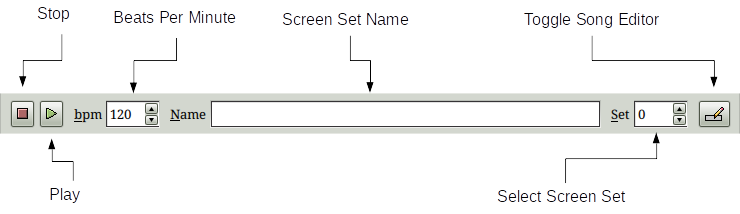
\includegraphics[scale=0.75]{pattern-window-bottom-panel-items.png}
   \caption{Patterns Panel, Bottom Panel Items}
   \label{fig:pattern_window_bottom_panel_items}
\end{figure}

   \begin{enumber}
      \item \textbf{Stop}
      \item \textbf{Play}
      \item \textbf{bpm}
      \item \textbf{Name}
      \item \textbf{Set}
      \item \textbf{Toggle Song Editor}
   \end{enumber}

   \setcounter{ItemCounter}{0}      % Reset the ItemCounter for this list.

   \itempar{Stop}{pattern!stop}
   The red squarebutton stops the playback of the song and all its patterns.
   It is not clear if it also sends MIDI Off messages on all notes.
   \index{keys!esc (stop)}
   The keystroke for stopping playback is the \texttt{Escape} character.

   \itempar{Play}{pattern!Play}
   The green triangular button starts the playback of the whole song.
   \index{keys!space (play)}
   The keystroke for starting playback is the \texttt{Space} character.

   \itempar{bpm}{pattern!bpm}
   The spin widget adjusts the "Beats Per Minute" or BPM value.  The
   range of this field is from 20 bpm to 500 bpm, with a default value of
   120 bpm.
   Although this field looks editable, it is not.  Most keystrokes
   that are entered actually toggle one of the pattern boxes.
   However, the following keys can also modify the BPM in small increments:
   \index{keys!semicolon} The \texttt{semicolon} reduces the BPM;
   \index{keys!apostrophe} The \texttt{apostrophe} increases the BPM.

   \itempar{Name}{pattern!set name}
   Each of the 32 available screen sets can be given a name by entering it
   into this field.

   \textbf{Bug:}
   \index{bugs!set name has side-effect}
   While one is typing in the name of the set in this field, the keystrokes
   will affect the panel window, causing playback to start and pattern
   boxes to be toggled!

   \itempar{Set}{pattern!set number}
   This spin widget selects the current screen set.  The values in this
   field range from 0 to 31, and default to 0.
   Although this field looks editable, it is not.

   \textbf{Bug:}
   \index{bugs!set number has side-effect}
   While one is typing in the number of the set in this field, the keystrokes
   will affect the panel window as well.

   \itempar{Toggle Song Editor}{pattern!toggle song editor}
   Pressing this button toggles the presence on-screen of the Song
   Editor.

%-------------------------------------------------------------------------------
% vim: ts=3 sw=3 et ft=tex
%-------------------------------------------------------------------------------


% Pattern Editor

%-------------------------------------------------------------------------------
% seq24_pattern_editor
%-------------------------------------------------------------------------------
%
% \file        seq24_pattern_editor.tex
% \library     Documents
% \author      Chris Ahlstrom
% \date        2015-07-19
% \update      2015-08-08
% \version     $Revision$
% \license     $XPC_GPL_LICENSE$
%
%     Provides the concepts.
%
%-------------------------------------------------------------------------------

\section{Pattern Editor}
\label{sec:seq24_pattern_editor}

   The \textsl{Seq24 Pattern Editor} is used to edit and preview a pattern,
   as well as to configure its buss and channel settings.

\begin{figure}[H]
   \centering 
   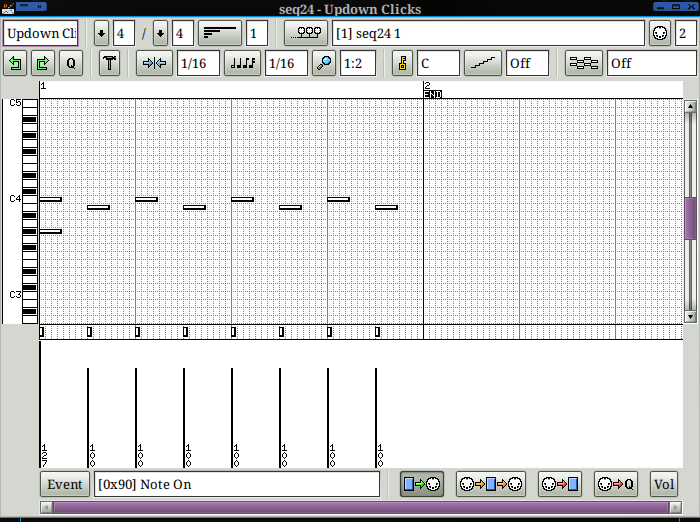
\includegraphics[scale=0.75]{pattern/pattern-edit-window.png}
   \caption{Pattern Edit Window}
   \label{fig:pattern_edit_window}
\end{figure}

   This dialog is quite complex.
   For exposition, we break it into a first panel, a second panel, a
   bottom panel, and a piano-roll/events section.

   \begin{enumber}
      \item \textbf{First Panel}
      \item \textbf{Second Panel}
      \item \textbf{Piano-Roll/Events Panel}
      \item \textbf{Bottom Panel}
   \end{enumber}

\subsection{Pattern Editor / First Panel}
\label{subsec:seq24_pattern_editor_first}

   The top bar of the Pattern (sequence) Editor lets you change the name of
   the pattern, the time signature of the piece, how long the loop is, and
   some other configuration items.

\begin{figure}[H]
   \centering 
   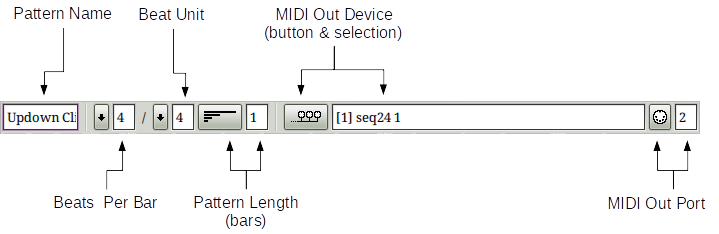
\includegraphics[scale=0.75]{pattern/pattern-edit-first-panel-items.png}
   \caption{Pattern Editor, First Panel Items}
   \label{fig:pattern_editor_first_panel_items}
\end{figure}

   \begin{enumber}
      \item \textbf{Pattern Name}
      \item \textbf{Beats Per Bar}
      \item \textbf{Beat Unit}
      \item \textbf{Pattern Length}
      \item \textbf{MIDI Out Device}
      \item \textbf{MIDI Out Port}
   \end{enumber}

   \setcounter{ItemCounter}{0}      % Reset the ItemCounter for this list.

   \itempar{Pattern Name}{pattern editor!name}
   Provides the name of the pattern.
   This name should be short and memorable.
   It is displayed in the Patterns window.

   \itempar{Beats Per Bar}{pattern editor!beats/bar}
   Part of the time signature, and specifies the number of beat units per bar.
   The possible values range from 1 to 16.

   \itempar{Beat Unit}{pattern editor!beat unit}
   Part of the time signature, and specifies the size of the beat unit:
   1 for whole notes; 2 for half notes; 4 for quarter notes; 8 for eight notes;
   and 16 for sixteenth notes.

   \itempar{Pattern Length}{pattern editor!progress}
   Sets the length of the current pattern, in measures.
   The possible values range from 1 to 16, then 32, and 64.

   \textsl{(It would sure be nice to have a value that represents
   "indefinite", so that the loop or pattern would be more like a track,
   and perhaps not be repeatable.)}

   \itempar{MIDI Out Device}{pattern editor!midi out device}
   This setting specifies one of the 16 MIDI output busses provided by
   \textsl{Seq24}.  The settings look a lot like
   \figureref{fig:pattern_window_right_click_midi_bus}.

   \itempar{MIDI Out Port}{pattern editor!midi out port}
   This settings select the MIDI output channel, or port.
   The possible values range from 1 to 16.

\subsection{Pattern Editor / Second Panel}
\label{subsec:seq24_pattern_editor_second}

   The second panel of the Pattern Editor provides a number of additional
   settings.

\begin{figure}[H]
   \centering 
   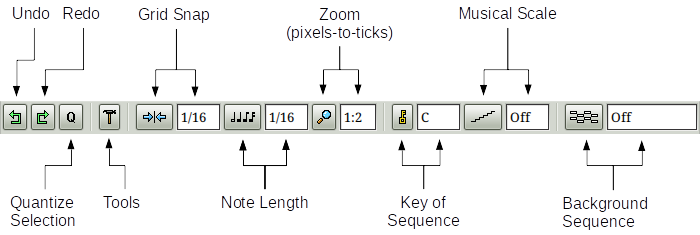
\includegraphics[scale=0.75]{pattern/pattern-edit-second-panel-items.png}
   \caption{Pattern Editor, Second Panel Items}
   \label{fig:pattern_editor_main_panel_items}
\end{figure}

   \begin{enumber}
      \item \textbf{Undo}
      \item \textbf{Redo}
      \item \textbf{Quantize Selection}
      \item \textbf{Tools}
      \item \textbf{Grid Snap}
      \item \textbf{Note Length}
      \item \textbf{Zoom}
      \item \textbf{Key of Sequence}
      \item \textbf{Musical Scale}
      \item \textbf{Background Sequence}
   \end{enumber}

   \setcounter{ItemCounter}{0}      % Reset the ItemCounter for this list.

   \itempar{Undo}{pattern editor!undo}
   The Undo button will roll back any changes to the pattern from this
   session.
   It will roll back one change each time it is pressed.
   It is not certain what the undo limit is, however.
   \index{keys!ctrl-z}
   Pressing \texttt{Ctrl-Z} is the same as using the \textbf{Undo} button.

   \itempar{Redo}{pattern editor!redo}
   The Redo button will restore any undone changes to the pattern from this
   session.
   It will restore one change each time it is pressed.
   It is not certain what the redo limit is, however.
   There doesn't seem to be a "Redo" key.

   \itempar{Quantize Selection}{pattern editor!quantize}
   Pressing this button will quantize the selected events, presumably as per
   the \textbf{Grid Snap} setting.

   \itempar{Tools}{pattern editor!tools}
   This button brings up a nested menu of tools for modifying selected
   events and notes.

\begin{figure}[H]
   \centering 
   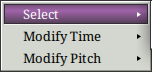
\includegraphics[scale=0.75]{pattern/tools-first-menu.png}
   \caption{Tools, Context Menu}
   \label{fig:pattern_editor_tools_first_menu}
\end{figure}

   \begin{enumber}
      \item \textbf{Select}
      \item \textbf{Modify Time}
      \item \textbf{Modify Pitch}
   \end{enumber}

   $\bullet$ \textbf{Select} provides two sets of selections for notes:
   \begin{itemize}
      \item \textbf{All Notes}, which selects all notes in the pattern;
         Note that \index{keys!ctrl-a} \texttt{Ctrl-A} will also select
         all of the events in the pattern editor.
      \item \textbf{Inverse Notes}, which inverts the selection of notes.
   \end{itemize}

   Other event-selection actions are provided:

   \begin{itemize}
      \item \index{left click}
         Pressing the left button on a note or a event deselects all other
         notes or events, and selects the item clicked on.
      \item \index{ctrl left click}
         Pressing the \texttt{Ctrl} key and the left button on a note or a
         event \textsl{adds} that event to the selection.
      \item \index{left click drag}
         Pressing the left mouse button and dragging also lets one
         select multiple events and notes.
      \item \index{ctrl left click drag}
         Pressing the \texttt{Ctrl} while left-click+dragging lets one
         make additional selections of multiple events and notes.
   \end{itemize}

   $\bullet$ \textbf{Modify Time} offers two ways to tweak the timing of the
   selected note:
   \textbf{Quantize Selected Notes}, which quantizes the selected
   notes, presumably the same way as the \textbf{Quantize} ("\textbf{Q}")
   button; \textbf{Tighten Selected Notes}, which presumably is a less
   strict form of quantization.
   TODO: \index{"todo!what is tighten"} Need more information about this.

   $\bullet$ \textbf{Modify Pitch} has only one entry by default,
   \textbf{Transpose Selected} (not shown).
   Selecting the \textbf{Transpose Selected} entry
   brings up the following sub-menu:

\begin{figure}[H]
   \centering 
   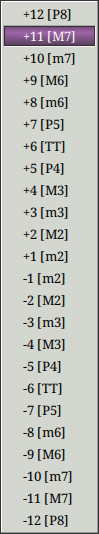
\includegraphics[scale=0.75]{pattern/tools-transpose-selected-menu.png}
   \caption{Tools, Transpose Selected Values}
   \label{fig:pattern_editor_tools_transpose_selected_menu}
\end{figure}

   $\bullet$ If the user has selected a
   \textbf{Musical Scale} setting other than \textbf{Off},
   then \textbf{Modify Pitch} has two entries:
   \textbf{Transpose Selected}, discussed above, plus
   another sub-menu,
   \textbf{Harmonic Transpose Selected}, which makes sure that all
   transpositions stay on the selected scale.

\begin{figure}[H]
   \centering 
   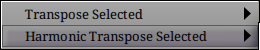
\includegraphics[scale=0.75]{pattern/tools-transpose-and-harmonic-selected-menu.png}
   \caption{Tools, Two "Transpose" Menus}
   \label{fig:pattern_editor_tools_two_transpose_menus}
\end{figure}

   Remember that only the 
   \textbf{Transpose Selected} entry is shown if the \textbf{Musical Scale}
   setting is \textbf{Off}.

   Selecting the \textbf{Harmonic Transpose Selected} entry brings up the
   following sub-menu:

\begin{figure}[H]
   \centering 
   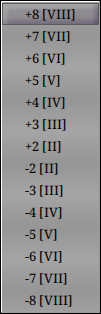
\includegraphics[scale=0.75]{pattern/tools-harmonic-transpose-selected-menu.png}
   \caption{Tools, Harmonic Transpose Selected Values}
   \label{fig:pattern_editor_tools_harmonic_transpose_menu}
\end{figure}

   Again, the harmonic-transpose option will not be available unless a scale
   has been selected.

   \itempar{Grid Snap}{pattern editor!grid snap}
   Grid snap selects where the notes will be drawn.
   The following values are supported:
   1, 1/2, 1/4, 1/8, 1/16, 1/32, 1/64, and 1/128.
   Additional values are also supported:
   1/3, 1/6, 1/12/, 1/24, 1/48, 1/96, and 1/192.

   \itempar{Note Length}{pattern editor!note length}
   Note Length determines what size they will be.
   Like the \textbf{Grid Snap} values,
   the following values are supported:
   1, 1/2, 1/4, 1/8, 1/16, 1/32, 1/64, and 1/128.
   Additional values are also supported:
   1/3, 1/6, 1/12/, 1/24, 1/48, 1/96, and 1/192.

   \itempar{Zoom}{pattern editor!zoom}
   Zoom is the relation between MIDI pixels and ticks, written as
   "pixels:ticks.
   For example, 1:4 = 4 ticks per pixel.
   Supported values are 1:1, 1:2, 1:4, 1:8, 1:16, and 1:32.

   \itempar{Key of Sequence}{pattern editor!key}
   Selects the desired key for the pattern.  The following scales are
   supported:  C, C\#, D, D\#, E, F, F\#, G, G\#, A, A\#, and B.

   \itempar{Musical Scale}{pattern editor!scale}
   Selects the desired scale for the pattern.
   Only the following values are supported: Off, Major, and Minor.

   One can select which \textbf{Musical Scale} and
   \textbf{Key} the piece is in,
   and \textsl{Seq24} will grey out those keys on the piano-roll that
   are \textsl{not} in the key.
   This effect is shown for the C Major scale in the following figure:

\begin{figure}[H]
   \centering 
   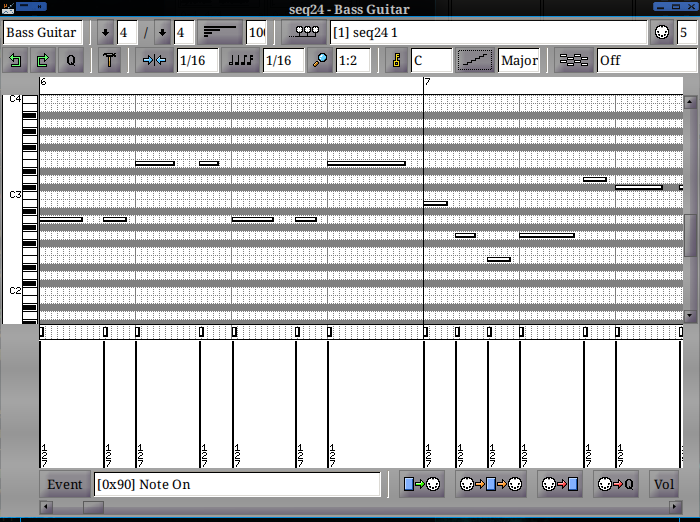
\includegraphics[scale=0.75]{pattern/major-scale-masking.png}
   \caption{C Major Scale Masking}
   \label{fig:pattern_editor_major_scale_masking}
\end{figure}

   This feature makes it a bit easier to stay in key while playing and
   recording.

   \itempar{Background Sequence}{pattern editor!background sequence}
   One can select another pattern to draw on the background to help with
   writing corresponding parts.
   The button brings up a small menu with values of \textbf{Off} and
   \textbf{[0]}.  Presumably, the 0 is a set number.  Under that entry, a
   menu like the following appears.

\begin{figure}[H]
   \centering 
   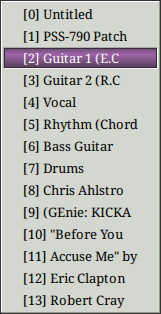
\includegraphics[scale=0.75]{pattern/background-sequence-menu.png}
   \caption{Sample Background Sequence Values}
   \label{fig:pattern_editor_background_sequence_menu}
\end{figure}

   Once the desired pattern is selected from that list, it appears as
   gray notes, along with the notes that are part of the pattern.  (Also
   note the orange selected notes and events in the following figure.)

\begin{figure}[H]
   \centering 
   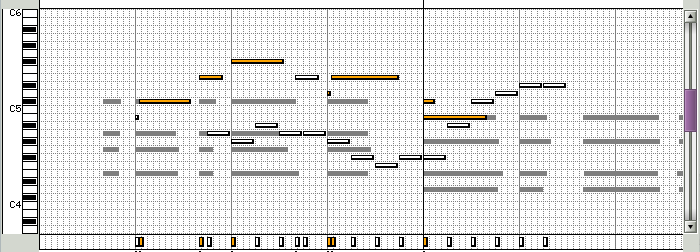
\includegraphics[scale=0.75]{pattern/background-sequence-notes.png}
   \caption{Background Sequence Notes}
   \label{fig:pattern_editor_background_sequence_notes}
\end{figure}

   The gray notes shown represent a rhythm pattern.

\subsection{Pattern Editor / Piano Roll}
\label{subsec:seq24_pattern_editor_piano_roll}

   The piano roll is the heart of the pattern (loop, sequence) editor.
   While it is very similar to note editors in other sequencers, it is a bit
   different in feel.  A good mouse with 3 or more buttons is practically a
   necessity for editing.  We tend to like the Logitech Marble Mouse, an
   ambidextrous USB trackball.  It has four bottons, and we use the
   \texttt{contrib/scripts/marblemouse} script to set up the left small
   button as a middle button.  The script merely makes the following call:

   \begin{verbatim}
      xmodmap -e "pointer = 1 8 3 4 9 6 7 2 5 10 11"
   \end{verbatim}

\subsubsection{Pattern Editor / Piano Roll Items}
\label{subsubsec:seq24_pattern_editor_piano_roll_items}

\begin{figure}[H]
   \centering 
   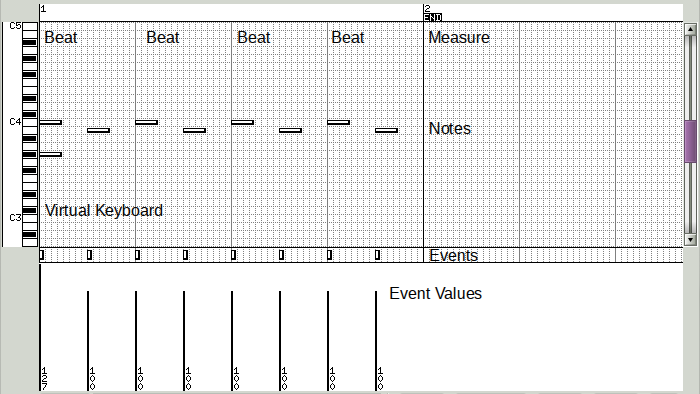
\includegraphics[scale=0.75]{pattern/pattern-edit-piano-roll-items.png}
   \caption{Pattern Editor, Piano Roll Items}
   \label{fig:pattern_editor_piano_roll_items}
\end{figure}

   \begin{enumber}
      \item \textbf{Beat}
      \item \textbf{Measure}
      \item \textbf{Virtual Keyboard}
      \item \textbf{Notes}
      \item \textbf{Events}
      \item \textbf{Event Values}
   \end{enumber}

   \setcounter{ItemCounter}{0}      % Reset the ItemCounter for this list.

   \itempar{Beat}{piano roll!beat}
   The light vertical lines represent the beats defined by the configuration
   for the pattern.

   \itempar{Measure}{piano roll!measure}
   The heavy vertical lines represent the measures defined by the
   configuration for the pattern.
   \index{pattern!end marker}
   Also note that the end of the pattern
   occurs at a measure, and is marked by a blocky \textbf{END} marker.

   \itempar{Virtual Keyboard}{piano roll!virtual keyboard}
   The virtual keyboard is a fairly powerful interface.  It shows,
   by shadowing, which note on the keyboard one will be drawing. It can be
   played with a mouse, to preview a short motif.
   It can show marks to indicate off-scale notes, to make them easy to
   avoid.

   \itempar{Notes}{piano roll!notes}
   Musical notes are indicated by short bars.  The bars provide a visual
   representation of the pitch of the note and the length of the notes.

   \itempar{Events}{piano roll!events}
   \index{events strip}
   The small (just a few pixels high) events strip shows discrete events,
   such as Note On and Note Off and their velocities, or various Controller
   items and their values.  We recommend not trying to edit or select events
   in that pane.

   \itempar{Event Values}{piano roll!event values}
   The events values for the currently selected category of events are shown
   in this window as vertical lines of a height proportional to the value.
   These values can be easily modified.

\subsubsection{Pattern Editor / Event Editing}
\label{subsubsec:seq24_pattern_editor_event_editing}

   Note editing is a bit different with \textsl{Seq24}, since it
   requires two mouse buttons in many cases.  There are some new
   laptop touchpads from FocalTech that have only one mouse button, and
   use positioning to determine if the click is a left- or right-click.
   The Linux drivers for this touchpad aren't sophisticated enough (as far
   as we know) to handle converting a two-fingered press properly.
   We've found that a good solution is to use a four-button USB trackball
   configued with an easy middle-button setup.
   It's easier than a touchpad, anyway.
   See the comments at the beginning of this section, too.

   Note that, if only a middle-button is needed, ctrl-left-button will
   simulate that button.

\paragraph{Editing Note Events}
\label{paragraph:seq24_pattern_editor_note_events}

   The Roll pane provides for a quite sophisticated set of note-editing
   actions.  Please study the following paragraphs carefully, ideally while
   trying them out in \textsl{Seq24}.

   \index{pattern editor!right click hold}
   \index{draw mode}
	In the note (grid/roll) panel, \textbf{holding}
	down the \textbf{right} mouse button will change the cursor
	to a pencil and put the editor into "draw" mode.
   
   \index{pattern editor!left click right hold}
   Then, while still \textbf{holding} the \textbf{right} mouse button, click
   the \textbf{left} mouse button to \textbf{insert} new notes.  Many people
   find this combination strange at first, but once one gets used to it, it
   becomes a very fast method of note manipulation.

   \index{pattern editor!right left hold drag}
   To increase the duration of the note(s), keep dragging the mouse (with
   both buttons held) rightward.
   \index{auto-notes}
   Note that, if one keeps dragging the mouse past the duration of a
   \index{beat unit}
   beat unit (e.g. a quarter note), then \textsl{multiple} notes are drawn,
   each one being the duration of a beat unit.  This \textsl{auto-note}
   facility can be convenient.
   
   However, if one wants a \textsl{single long note}, first draw the
   short note, and then use one of the operations described in the next
   paragraph to change the length of the note.  These operations also caused
   the note to be selected.

   \index{pattern editor!ctrl left click}
   \index{pattern editor!middle click}
   Pressing the \textbf{middle} mouse button \textbf{\textsl{or}}
   pressing the \textbf{ctrl left} mouse button tandem will let one change 
	the length of the note. 
   If more than one note is selected, then the length of all selected notes
   is changed.
   
   \textbf{Warning}:  If one reduces the length of a note by more than its
   current length, the note will end up "infinitely" long.

   \index{pattern editor!left click drag}
	The \textbf{left} mouse button lets you select multiple events 
   which can then be clicked and moved,
   \index{pattern editor!cut}
   \index{keys!ctrl-x} cut (\texttt{Ctrl-X}), 
   \index{pattern editor!copy}
   \index{keys!ctrl-c} copy (\texttt{Ctrl-C}),
   \index{pattern editor!paste}
   \index{keys!ctrl-v} or pasted (\texttt{Ctrl-V}).
   When the notes are selected,
   \index{pattern editor!delete}
   \index{keys!del} you can delete them with the \texttt{Delete} key.

   \index{ctrl left click drag}
   Pressing the \texttt{Ctrl} while left-click+dragging lets one
   make additional selections of multiple events and notes.

   For the appearance of selected events (orange), see
   \figureref{fig:pattern_editor_selected_events}.

\begin{figure}[H]
   \centering 
   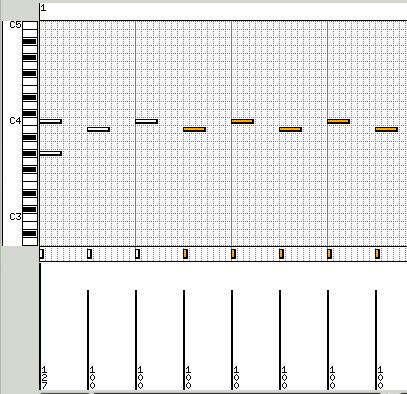
\includegraphics[scale=0.75]{pattern/pattern-edit-selected-events.png}
   \caption{Piano Roll, Selected Notes and Events}
   \label{fig:pattern_editor_selected_events}
\end{figure}

   \index{left click}
   Pressing the left button on a note or a event deselects all other notes
   or events, and selects the item clicked on.

   \index{ctrl left click}
   Pressing the \texttt{Ctrl} key and the left button on a note or a event
   \textsl{adds} that event to the selection.

   \index{left click drag}
   Note that pressing the left mouse button and dragging also lets one
   select multiple events and notes.
   \index{ctrl left click drag}
   Pressing the \texttt{Ctrl} while left-click+dragging lets one
   make additional selections of multiple events and notes.

   The \textbf{Tools} button described in
   \sectionref{subsec:seq24_pattern_editor_second} can also be used to
   modify selections.

   \index{keys!ctrl-a}
   \texttt{Ctrl-A} will select all of the events in the pattern editor.

   \index{pattern editor!ctrl left click}
   \index{pattern editor!middle click}
   Pressing the \textbf{middle} mouse button \textbf{\textsl{or}}
   pressing the \textbf{ctrl left} mouse button tandem will let one change 
	the length of the note. 
   If more than one note is selected, then the length of all selected notes
   is changed.

   \index{pattern editor!event stretch}
   \index{pattern editor!shift middle click drag}
   Once a selection of notes is made, one can use the
   Shift-middle-click+drag sequence over the selected notes to
   draw a box beyond the extent of the notes.  When the mouse is released,
   each of the events is moved and lengthed to be proporationally longer to
   fit exactly within the box one drew.
   This feature is called \textsl{event stretch}.

   \index{pattern editor!event compression}
   If the box that was drawn was shorter than the original extent of the
   notes, then the notes move and shrink proportionally to occupy the
   smaller box.
   This feature is called \textsl{event compression}.
   
   \textbf{Warning}:  If one reduces the length of a note by more than its
   current length, the note will end up "infinitely" long.

   \index{pattern editor!left click drag}
	The \textbf{left} mouse button lets you select multiple events 
   which can then be clicked and moved,
   \index{pattern editor!cut}
   \index{keys!ctrl-x}
   cut (\texttt{Ctrl-X}), 
   \index{pattern editor!copy}
   \index{keys!ctrl-c}
   copy (\texttt{Ctrl-C}),
   \index{pattern editor!paste}
   \index{keys!ctrl-v}
   or pasted (\texttt{Ctrl-V}).
   When the notes are selected,
   \index{pattern editor!delete}
   \index{keys!del}
   you can delete them with the \texttt{Delete} key.

\paragraph{Editing Other Events}
\label{paragraph:seq24_pattern_editor_other_events}

%  Left-click or right-click on events in the event strip (directly under
%  the piano roll grid) will allow you to add/select/move 
%  MIDI events (including note on/off messages) somewhat like the 
%  piano grid.

   \index{event strip}
   Note On and Note Off events appear as small squares in the event strip,
   along with a black vertical bar with a height proportional to the
   velocity of the note event, plus a numeric representation of that value.
   Note events do not need to be inserted in the event strip.
   (\textsl{Note events can be inserted there, but they end up as short
   events of the lowest possible note, 0 or C1, and they don't have a Note
   Off event.  So don't do that!})

   Other events can be inserted via the event strip.  To do that, first
   select the kind of event to insert using the \textbf{Event} button in the
   bottom panel.  The place the mouse cursor in the event strip.
   Right-click to make the drawing pencil appear at the exact spot where the
   event must go.  While holding the right button, click the left button.
   A small square for the event should appear.

   Should one want more of the same event, continue to hold both buttons and
   drag the mouse.  One event should appear at each beat position (e.g. at
   each 16th note position) that is crossed.

   To move the event(s) to a different spot, select it or them via the left
   button.  Then drag it or them to where one wants them.
   \index{todo!high precision events}
   \textsl{Note: it
   is currently not possible to move them to positions smaller than the
   beat size.  Is there a way to do it?}

   Once the event positions are set, the next step is to modify the
   data values of the events.

   \index{event data}
	The event value (data) editor (directly under the event strip) is used 
	to change note velocities, channel pressure, control codes,
	patch select, etc.
   \index{event data editor!draw}
   \index{event data editor!left click}
   \index{event data editor!right click}
   \index{event data editor!middle click}
   Just left-click+drag the mouse across the window to draw a line.  The
   values will match that line.  
   middle-click+drag and right-click+drag also
   draw the value line.

   \textbf{Bug:}
   \index{bugs!event editing can fail}
   Sometimes the editing of event values in the event data section will not work.
   The workaround is to do a \texttt{Ctrl-A}, and the click in the roll
   to deselect the selection; that makes the event value editing work again.
   
   \index{event data editor!mouse wheel}
   Any events that are selected in the piano roll or event strip can have
   their values modified with the mouse wheel.

\subsection{Pattern Editor / Bottom Panel}
\label{subsec:seq24_pattern_editor_bottom}

   The bottom panel of the Pattern Editor provides for selecting events for
   viewing and edition, and the MIDI playback, pass-through, and recording
   options of \textsl{Seq24}.

\begin{figure}[H]
   \centering 
   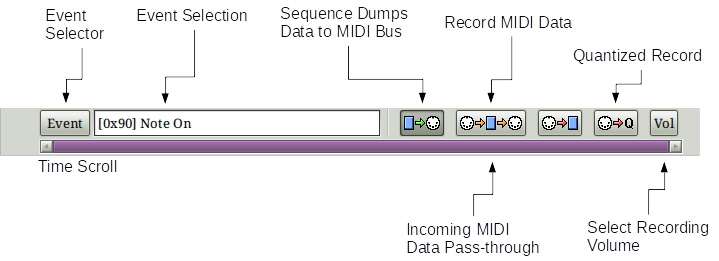
\includegraphics[scale=0.75]{pattern/pattern-edit-bottom-panel-items.png}
   \caption{Pattern Editor, Bottom Panel Items}
   \label{fig:pattern_editor_bottom_panel_items}
\end{figure}

   \begin{enumber}
      \item \textbf{Event Selector}
      \item \textbf{Event Selection}
      \item \textbf{Time Scroll}
      \item \textbf{Data To MIDI Buss}
      \item \textbf{MIDI Data Pass-Through}
      \item \textbf{Record MIDI Data}
      \item \textbf{Quantized Record}
      \item \textbf{Select Recording Volume}
   \end{enumber}

   \setcounter{ItemCounter}{0}      % Reset the ItemCounter for this list.

   \itempar{Event Selector}{pattern editor!event selector}
   This button brings up the following context menu, so that the user can
   select the category of events to view and edit.

\begin{figure}[H]
   \centering 
   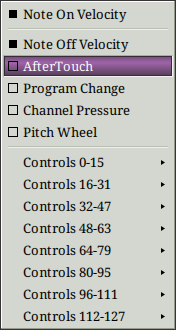
\includegraphics[scale=0.75]{pattern/event-context-menu.png}
   \caption{Pattern Editor, Event Button Context Menu}
   \label{fig:pattern_editor_bottom_event_context_menu}
\end{figure}

   The sub-menus of this context menu show 128 controller messages,
   so we won't try to show all of them here.

   These sub-menus can be modified, as far as we know, by editing
   the file \texttt{\$HOME/.seq24usr}, to make it match your instrument.
   See \sectionref{sec:seq24_usr_file}.

   \itempar{Event Selection}{pattern editor!event selection}
   Shows the selection event, with its number shown in hexadecimal notation,
   and the name of the event shown.

   \itempar{Time Scroll}{pattern editor!time scroll}
   Allows one to pan through the whole pattern, if it is too long to fit in
   the window.

   \itempar{Data To MIDI Buss}{pattern editor!data to midi buss}
   Activating this button will cause the pattern to be output to the MIDI
   output buss, which will normally be connected to a software or hardware
   synthesizer, to be heard.

   \itempar{MIDI Data Pass-Through}{pattern editor!midi data pass-through}
   Activating this button will route incoming MIDI data through
   \textsl{Seq24}, which will then write it to the MIDI output buss.

   \itempar{Record MIDI Data}{pattern editor!record midi data}
   Activating this button will route incoming MIDI data into
   \textsl{Seq24}, which will then save the data to its buffer, and also
   display the new information (notes) in the piano roll view.

   \itempar{Quantized Record}{pattern editor!quantized record}
   Activating this button will also cause MIDI data to be recorded, but it
   will be quantized on the fly before saving it.

   \itempar{Vol}{pattern editor!vol}
   This button allows controlling the volume of the recording.

\begin{figure}[H]
   \centering 
   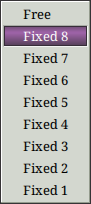
\includegraphics[scale=0.75]{pattern/vol-context-menu.png}
   \caption{Pattern Recording Volume Menu}
   \label{fig:pattern_edit_recording_volume_menu}
\end{figure}

   The values provided are:
   Free, Fixed 8, Fixed 7, Fixed 6, Fixed 5, Fixed 4, Fixed 3,
   Fixed 2, and Fixed 1.
   TODO: \index{todo!explain recording volume}
   We need to figure what these mean!

%-------------------------------------------------------------------------------
% vim: ts=3 sw=3 et ft=tex
%-------------------------------------------------------------------------------


% Song Editor

%-------------------------------------------------------------------------------
% seq24_song_editor
%-------------------------------------------------------------------------------
%
% \file        seq24_song_editor.tex
% \library     Documents
% \author      Chris Ahlstrom
% \date        2015-07-19
% \update      2015-07-21
% \version     $Revision$
% \license     $XPC_GPL_LICENSE$
%
%     Provides the concepts.
%
%-------------------------------------------------------------------------------

\section{Song Editor}
\label{sec:seq24_song_editor}

   The \textsl{Seq24 Song Editor} is used to combine all of the patterns
   into a complete tune.  It works by showing one row per
   pattern/loop/sequence in numbered columns, and the placement of each
   pattern at various musical bars in the song.

   In \textsl{Seq24} parlance, the Song Editor creates a
   \textsl{performance}.

\begin{figure}[H]
   \centering 
   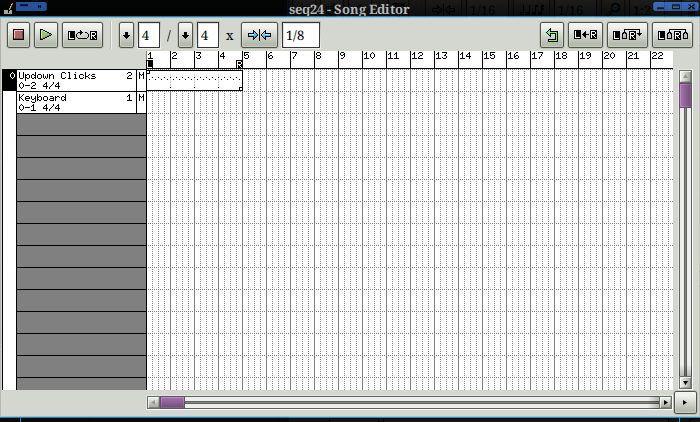
\includegraphics[scale=0.75]{song-editor/song-editor-window.png}
   \caption{Song Editor Window}
   \label{fig:song_editor_window}
\end{figure}

   This dialog is not too complex, but
   for exposition, we break it into a top panel and the rest of the window.

\subsection{Song Editor / Top Panel}
\label{subsec:seq24_song_editor_top}

   The top panel provides quick access to song-playback actions and
   configuration.

\begin{figure}[H]
   \centering 
   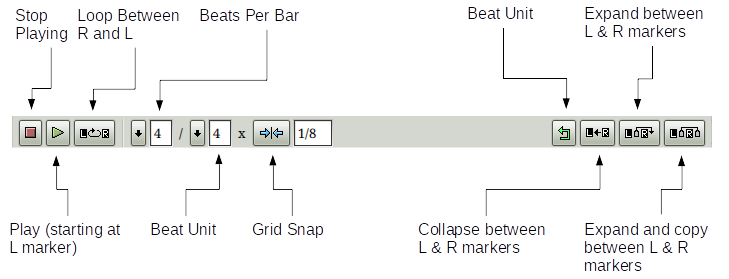
\includegraphics[scale=0.75]{song-editor/song-editor-top-panel-items.png}
   \caption{Song Editor / Top Panel Items}
   \label{fig:song_editor_top_panel_items}
\end{figure}

   \begin{enumber}
      \item \textbf{Stop}
      \item \textbf{Play}
      \item \textbf{Loop}
      \item \textbf{Beats Per Bar}
      \item \textbf{Beat Unit}
      \item \textbf{Grid Snap}
      \item \textbf{Undo}
      \item \textbf{Collapse}
      \item \textbf{Expand}
      \item \textbf{Expand and copy}
   \end{enumber}

   \setcounter{ItemCounter}{0}      % Reset the ItemCounter for this list.

   \itempar{Stop}{song editor!stop}
   Stops the playback of the song.
   \index{keys!esc (stop)}
   The keystroke for stopping playback is the 'Escape' character.

   \itempar{Play}{song editor!play}
   \index{L marker}
   Starts the playback of the song, starting at the \textbf{L marker}.
   \index{keys!space (play)}
   The keystroke for starting playback is the 'Space' character.

   \itempar{Loop}{song editor!loop}
   \index{L marker}
   \index{R marker}
   Play the song, looped between the \textbf{L marker} and the
   \textbf{R marker}.
   This button is a state button, and its appearance indicates when it is
   depressed, and thus active.
   If this button is deactivated during playback, then playback will
   continue past the \textbf{R marker}.

   \itempar{Beats Per Bar}{song editor!beats/bar}
   Part of the time signature, and specifies the number of beat units per bar.
   The possible values range from 1 to 16.

   \itempar{Beat Unit}{song editor!beat unit}
   Part of the time signature, and specifies the size of the beat unit:
   1 for whole notes; 2 for half notes; 4 for quarter notes; 8 for eight notes;
   and 16 for sixteenth notes.

   \itempar{Grid Snap}{song editor!grid snap}
   Grid snap selects where the patterns will be drawn.
   Unlike the \textbf{Grid Snap} of the Pattern Editor, the units
   of the Song Editor snap value are in fractions of a measure length.
   The following values are supported:
   1/1, 1/2, 1/4, 1/8, 1/16, and 1/32.

   \itempar{Undo}{song editor!undo}
   The Undo button will roll back the last change in the layout of a
   pattern.  Each time it is clicked, the most recent change will be undone.
   It will roll back one change each time it is pressed.
   It is not certain what the undo limit is, however.
   There is no Redo button in the Song Editor.

   \itempar{Collapse}{song editor!collapse}
   This button collapses the song between the \textbf{L marker} and the
   \textbf{R marker}.
   What this means is that, if there is song material (patterns) before the
   \textbf{L marker} and after the \textbf{R marker},
   and the \textbf{Collapse} button is
   pressed, any song material between the L and R markers is wiped out, and
   the song material after the \textbf{R marker} is moved leftward to
   the \textbf{L marker}.

   Collapsing occurs in all tracks present in the Song Editor.

   \itempar{Expand}{song editor!expand}
   This button expands the song between the
   \textbf{L marker} and the \textbf{R marker}.
   It inserts blank space between these markers, moving the song material
   that is after the \textbf{R marker}
   to the right by the duration of the blank space.

   Expansion occurs in all tracks present in the Song Editor.

   \itempar{Expand and copy}{song editor!expand and copy}
   This button expands the song between the \textbf{L marker} and the
   \textbf{R marker} much like the \textbf{Expand} button.
   However, it also copies the original data that is present after the
   \textbf{R marker}, and pastes it into the newly-available space between
   the L and R markers.

\subsection{Song Editor / Arrangement Panel}
\label{subsec:seq24_song_editor_arrangement_panel}

   The arrangement panel is the middle section shown in
   \figureref{fig:song_editor_window}.  Here, we zero in on its many
   features.

   The following figure is taken from a conventional MIDI file, with a few
   long tracks, rather than a large number of smaller patterns.  In other
   words, the patterns used here are very long, and used only once in the
   song.
   
   We might need to provide an example that shows off \textsl{Seq24}'s
   pattern features better, at some point.

\begin{figure}[H]
   \centering 
   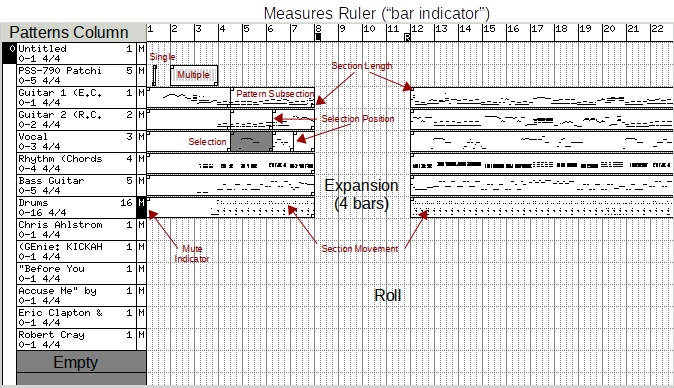
\includegraphics[scale=0.75]{song-editor/song-editor-window-full-items.png}
   \caption{Song Editor Arrangement Panel, Annotated}
   \label{fig:song_editor_window_full_items}
\end{figure}

   \index{measures ruler}
   It consists of a \textsl{measures ruler} (bar indicator) at the top, a
   numbered patterns column at the left with a muting indicator, and the
   grid or roll section.  There are a lot of hidden details in the
   arrangement panel, as the figure shows.  Here are the main sections we
   will deal with:

   \begin{enumber}
      \item \textbf{Patterns Column}
      \item \textbf{Roll}
      \item \textbf{Measures Ruler}
   \end{enumber}

   These items are discussed in the following sections.

\subsubsection{Song Editor / Arrangement Panel / Patterns Column}
\label{subsubsec:seq24_song_editor_arrangement_panel_patterns_column}

   Here are the items to note in the patterns column:

   \begin{enumber}
      \item \textbf{Number}.
         Not yet sure what the number on the left means.
         The number of the screen set?
      \item \textbf{Title}.
         \index{pattern!title}
         \index{pattern!name}
         The title is the name of the pattern, for easy reference.
      \item \textbf{Channel}.
         \index{pattern!channel}
         The channel number appears at the right of the title.
      \item \textbf{Span}.
         \index{pattern!span}
         This pair of numbers shows the starting measure of the pattern and
         the measure just after the end of the pattern.
      \item \textbf{Beat}.
         \index{pattern!beat}
         This pair of numbers is the standard time-signature of the pattern.
      \item \textbf{Mute Indicator}.
         \index{song editor!mute indicator}
         The letter M is in a black box if the track/pattern is muted, and a
         white box if it is unmuted.
      \item \textbf{Empty}.
         Empty tracks are indicated by a dark-gray filling.
   \end{enumber}

   The patterns column shows a list of all of the patterns that have been
   created in the current song.  Each pattern in this list has a track of
   pattern layouts associated with it in the Roll section.

   \index{patterns column!left click}
   Left-clicking on the pattern name or the "M" button toggles the muting
   status of the track.

   \index{patterns column!right click}
   Right-clicking on the pattern name or the "M" button brings up the same
   pattern editing menu as discussed in
   \sectionref{subsubsec:seq24_patterns_pattern_filled}.
   Recall that this context menu has the following entries:
   Edit..., Cut, Copy, Song, and Midi Bus.

\subsubsection{Song Editor / Arrangement Panel / Roll}
\label{subsubsec:seq24_song_editor_arrangement_panel_roll}

   The "Roll" section of the arrangement panel is where patterns or
   subsections are inserted, deleted, shrunk, lengthened, or moved.

   Here are the items to note in the Roll area:

   \begin{enumber}
      \item \textbf{Single}.
         In the diagram, under the word "Single", is a very small pattern.
         It is small because it consists only of some MIDI Program Change
         messages meant to set the programs on a Yamaha PSS-790 keyboard.
      \item \textbf{Multiple}.
         This items is the same pattern as in "Single", but dragged out for
         multiple repetitions, simply to show how even the shortest patterns
         can be easily replicated.
      \item \textbf{Pattern Subsection}.
         \index{song editor!middle click}
         \index{pattern subsection}
         Middle-clicking inside a pattern inserts a selection position
         marker in it, breaking the pattern into two equal pieces.
         We call each piece a \textsl{pattern subsection}.
         This division can be done over and over.
         (Note that, in the Song Editor, a middle-click
          \textsl{cannot} be simulated by ctrl-left-click.)
      \item \textbf{Selection Position}.
         A selection position is a marker that divides a pattern into two
         pieces, called \textsl{pattern subsections}.  This makes it easy to
         select smaller portions of a pattern for editing or deleting.  It
         is especially useful for making holes in a pattern.  There may be
         other uses of a selection position that we have not yet discovered.
      \item \textbf{Selection}.
         By clicking inside a pattern or a pattern subsection, it darkens to
         denote that it is selected.
         A pattern subsection can be deleted by the
         \index{keys!delete}
         Delete key, copied by the
         \index{keys!ctrl-c}
         \texttt{Ctrl-C} key, and then inserted (one or more times) by the
         \index{keys!ctrl-v}
         \texttt{Ctrl-V} key.  When inserted, each insert goes immediately
         after the current item or the previous insertion.  The same can be
         done for whole patterns.
      \item \textbf{Section Length}.
         Looking closely at the diagram where the arrows point, small
         squares in the corner of the patterns can be seen.  By grabbing
         that square with a left-click, the square can be moved horizontally
         to either lengthen or shorted the pattern or pattern subsection, if
         there is room to move in the desired direction.
         It doesn't matter if the item is selected or not.
      \item \textbf{Section Movement}.
         If, instead of grabbing the section length handle, one grabs inside
         the pattern or pattern subsection, that item can be moved
         horizontally, as long as their is room.  Or course, left-clicking
         inside the item will also cause it to show as selected.
      \item \textbf{Expansion}.
         Originally, all the long patterns of this song were continuous.
         But, by setting the L and R markers, and using the \textbf{Expand}
         button, we opened up some space in the song.
   \end{enumber}

   The \textsl{Seq24} help files refer to work in the Song Editor as the
   "Performance Edit" or "Performance Mode".  Adding a pattern in this
   window is a bit like adding a note in the Pattern Editor.
   One clicks, holds, and drags the mouse to insert a copy of the pattern
   associated with the row in which one is dragging.  The longer one drags,
   the more copies of the pattern that are inserted.

   \index{song editor!right click hold}
	Right-click on the arrangement panel (roll) to enter
   draw mode, and hold the button.

   \index{song editor!left click right hold}
   Then left-click the mouse to insert one copy of the pattern.  The
   inserted pattern will show up as a box with a tiny representation of the
   notes visible inside.  (Some patterns, however, can be less than a
   measure in length, resulting in a tiny box.)

   \index{song editor!right left hold drag}
   To keep adding more copies of the pattern, continue to hold both buttons
   and drag the mouse rightward.

   \index{song editor!middle click}
   Middle-click on a pattern to drop a new selection position into the
   pattern,
   \index{song editor!pattern subsection}
   which breaks the pattern into two equal \textsl{pattern subsections}.
   Each middle-click on the pattern adds a new selection position,
   halving the size of the subsections as more pattern subsections are
   added.

   \index{song editor!left click}
   When a pattern or a pattern subsection is left-clicked, it is marked as
   dark gray.
   \index{song editor!right left hold drag}
   When a right-left-hold-drag action is done in this gray area, the result
   is to \textsl{delete} that pattern section or subsection.
   \index{keys!delete}
   One can also hit the Delete key to \textsl{delete} that pattern section
   or subsection.

\subsubsection{Song Editor / Arrangement Panel / Measures Ruler}
\label{subsubsec:seq24_song_editor_arrangement_panel_measures_ruler}

   The \textsl{measures ruler} is the ruled and numbered section at the top
   of the arrangement panel.  It provides a place to put the left and right
   markers.  In the \textsl{Seq24} documentation, it is called the "bar
   indicator".

   \index{measures ruler!left-click}
   Left-click in the measures ruler to drop an
   \index{L anchor}
   \textbf{L anchor} on the measures ruler.
   \index{measures ruler!right-click}
   Right-click in the measures ruler to drop an
   \index{R anchor}
   \textbf{R anchor} on the measures ruler.

   Once these anchors are in place, then use
	the \textsl{Collapse} and \textsl{Expand} buttons to modify the
   placement of the pattern events.

   Note that the \textbf{L marker} serves as the start position for playback
   in the Song Editor.  One can change the start position only when the
   performance is not playing.

%-------------------------------------------------------------------------------
% vim: ts=3 sw=3 et ft=tex
%-------------------------------------------------------------------------------


% Man page

% %-------------------------------------------------------------------------------
% seq24_manpage
%-------------------------------------------------------------------------------
%
% \file        seq24_manpage.tex
% \library     Documents
% \author      Chris Ahlstrom
% \date        2015-07-21
% \update      2015-07-21
% \version     $Revision$
% \license     $XPC_GPL_LICENSE$
%
%     Provides the man page section of seq24-user-manual.tex.
%
%-------------------------------------------------------------------------------

\section{Seq24 Man Page}
\label{sec:seq24_man_page}

   This section presents the contents of the \textsl{Seq24} man page, but
   not exactly in \textsl{man} format.  Also, an item or two are shown that
   somehow didn't make it into the man page, and minor corrections and
   formatting tweaks were made.

   \textsl{Seq24} - Real time MIDI sequencer.

   \textsl{Seq24} is a real-time MIDI sequencer. It was created to provide a
   very simple interface for editing and playing MIDI 'loops'.

   \begin{verbatim}
       seq24 [OPTIONS] [FILENAME]
   \end{verbatim}

   \textsl{Seq24} accepts the following options, plus an optional name of a
   MIDI file.

   \setcounter{ItemCounter}{0}      % Reset the ItemCounter for this list.

   \optionpar{-h}{--help}
      Display a list of all command-line options.

   \optionpar{-v}{--version}
      Display the program version.

   \optionpar{N/A}{--file [filename]}
      Load MIDI file on startup.
      \textbf{Bug:}
      \index{bugs!--file option doesn't exist}
      This option does not exist.

   \optionpar{-m}{--manual\_alsa\_ports}
      \textsl{Seq24} won't attach ALSA ports.

   \optionpar{-s}{--showmidi}
      Dumps incoming MIDI to the screen.

   \optionpar{-p}{--priority}
      Runs at higher priority with FIFO scheduler.

   \optionpar{N/A}{--pass\_sysex}
      Passes any incoming SYSEX messages to all outputs.

   \optionpar{-i}{--ignore [number]}
      Ignore ALSA device [number].

   \optionpar{-k}{--show\_keys}
      Prints pressed key value.

   \optionpar{-x}{--interaction\_method [number]}
      Select the mouse interaction method.
      0 = seq24 (the default); and 1 = fruity loops method>

   \optionpar{-j}{--jack\_transport}
      \textsl{Seq24} will sync to JACK transport.

   \optionpar{-J}{--jack\_master}
      \textsl{Seq24} will try to be JACK master

   \optionpar{-C}{--jack\_master\_cond}
      JACK master will fail if there is already a master

   \optionpar{-M}{--jack\_start\_mode [x]}
      When \textsl{Seq24} is synced to JACK, the following play modes are
      available: 0 = live mode; and 1 = song mode, the default.

   \optionpar{-S}{--stats}
      Print statistics on the command-line while running.

   \optionpar{-U}{--jack\_session\_uuid [uuid]}
      Set the UUID for the JACK session.

   \texttt{\$HOME/.seq24rc} stores the user settings for \textsl{Seq24}.

   The old project homepage is at
   \url{http://www.filter24.org/seq24/} the new
   one is at \url{https://edge.launchpad.net/seq24/}.
   It is released under the GNU GPL license.

   \textsl{Seq24} was written by Rob C. Buse \url{mailto:seq24@filter24.org}
   and the \textsl{Seq24} team.

   This manual page was written by Dana Olson
   \url{mailto:seq24@ubuntustudio.com} with additions from Guido Scholz
   \url{mailto:guido.scholz@bayernline.de}.

   \begin{verbatim}
Version 0.9.2                   November 20 2010                       Seq24(1)
   \end{verbatim}

%-------------------------------------------------------------------------------
% vim: ts=3 sw=3 et ft=tex
%-------------------------------------------------------------------------------


% Building and debugging Seq24

% \input{yum_build}

\section{Summary}
\label{sec:summary}

   In summary, we can say that you will find \textsl{Seq24} intriguing.

   There are some topics that this document does not yet treat ...:

% References

%-------------------------------------------------------------------------------
% seq24_references
%-------------------------------------------------------------------------------
%
% \file        seq24_references.tex
% \library     Documents
% \author      Chris Ahlstrom
% \date        2015-07-19
% \update      2015-07-20
% \version     $Revision$
% \license     $XPC_GPL_LICENSE$
%
%     Provides the References section of yoshimi-seq24.tex.  Rather
%     than use the bibtex package, our small set of references uses a
%     simpler method.
%
%-------------------------------------------------------------------------------

\section{References}
\label{sec:seq24_references}

   The \textsl{Yoshimi} seq24 reference list.

\begin{thebibliography}{99}

   \bibitem{amsynth}
   amSynth team, Nick Dowell
   \emph{amSynth and Demos with Calf Effects.}
   \url{http://amsynth.com/amsynth.html}
   Includes links to demos and the source code.
   2015.

   \bibitem{bristol}
   Bristol team Nick Copeland
   \emph{Bristol: A Vintage Synthesizer Emulator}
   \url{http://www.linuxsynths.com/BristolPatchesDemos/bristol.html}
   2014.

   \bibitem{fluidsynth}
   FluidSynth team
   \emph{FluidSynth: A SoundFont Synthesizer}
   \url{http://www.fluidsynth.org/}
   2014.

   \bibitem{linuxsynths}
   LinuxSynths team, briandc@linuxsynths.com
   \emph{A Sonic Palette on the Linux Platform.}
   \url{http://www.linuxsynths.com/}
   2015.

   \bibitem{ljtutorial}
   Dave Phillips
   \emph{At the Sounding Edge: Introducing seq24.}
   \url{http://www.linuxjournal.com/article/8304}
   Linux Journal, May 12, 2005.

   \bibitem{midicvt}
   Chris Ahlstrom
   \emph{Extension of midicomp/midi2text to convert between MIDI and ASCII text format.}
   \url{https://github.com/ahlstromcj/midicvt}
   2015.

   \bibitem{seq24}
   Seq24 Team.
   \emph{The home site for the Seq24 looping sequencer.}
   \url{http://www.filter24.org/seq24/download.html}
   2010.

   \bibitem{timidity}
   Timidity++ Team.
   \emph{Download site for Timidity++ source code.}
   \url{http://sourceforge.net/projects/timidity/}
   2015.

   \bibitem{yoshimi}
   Yoshimi team \url{abrolag@users.sourceforge.net}
   \emph{The download site for the Yoshimi software synthesizer.}
   \url{http://yoshimi.sourceforge.net/}
   2015.

   \bibitem{yoshimi2}
   Yoshimi team
   \emph{The alternate location for the Yoshimi source-code.}
   \url{https://github.com/abrolag/yoshimi/}
   2015.

   \bibitem{yoshimidoc}
   Chris Ahlstrom
   \emph{A Yoshimi User Manual.}
   \url{https://github.com/ahlstromcj/yoshimi-doc/}
   2015.

   \bibitem{yoshimicook}
   Chris Ahlstrom
   \emph{A Yoshimi Cookbook.}
   \url{https://github.com/ahlstromcj/yoshimi-seq24/}
   2015.

   \bibitem{zynaddsubfx}
   Mark McCurry, Paul Nasca (ZynAddSubFX team)
   \emph{The download site for the ZynAddSubFX software synthesizer.}
   \url{http://zynaddsubfx.sourceforge.net/}
   2015.

\end{thebibliography}

%-------------------------------------------------------------------------------
% vim: ts=3 sw=3 et ft=tex
%-------------------------------------------------------------------------------


\printindex

\end{document}

%-------------------------------------------------------------------------------
% vim: ts=3 sw=3 et ft=tex
%-------------------------------------------------------------------------------
